\documentclass[twoside]{book}

% Packages required by doxygen
\usepackage{calc}
\usepackage{doxygen}
\usepackage{graphicx}
\usepackage[utf8]{inputenc}
\usepackage{makeidx}
\usepackage{multicol}
\usepackage{multirow}
\usepackage{textcomp}
\usepackage[table]{xcolor}

% Font selection
\usepackage[T1]{fontenc}
\usepackage{mathptmx}
\usepackage[scaled=.90]{helvet}
\usepackage{courier}
\usepackage{amssymb}
\usepackage{sectsty}
\renewcommand{\familydefault}{\sfdefault}
\allsectionsfont{%
  \fontseries{bc}\selectfont%
  \color{darkgray}%
}
\renewcommand{\DoxyLabelFont}{%
  \fontseries{bc}\selectfont%
  \color{darkgray}%
}

% Page & text layout
\usepackage{geometry}
\geometry{%
  a4paper,%
  top=2.5cm,%
  bottom=2.5cm,%
  left=2.5cm,%
  right=2.5cm%
}
\tolerance=750
\hfuzz=15pt
\hbadness=750
\setlength{\emergencystretch}{15pt}
\setlength{\parindent}{0cm}
\setlength{\parskip}{0.2cm}
\makeatletter
\renewcommand{\paragraph}{%
  \@startsection{paragraph}{4}{0ex}{-1.0ex}{1.0ex}{%
    \normalfont\normalsize\bfseries\SS@parafont%
  }%
}
\renewcommand{\subparagraph}{%
  \@startsection{subparagraph}{5}{0ex}{-1.0ex}{1.0ex}{%
    \normalfont\normalsize\bfseries\SS@subparafont%
  }%
}
\makeatother

% Headers & footers
\usepackage{fancyhdr}
\pagestyle{fancyplain}
\fancyhead[LE]{\fancyplain{}{\bfseries\thepage}}
\fancyhead[CE]{\fancyplain{}{}}
\fancyhead[RE]{\fancyplain{}{\bfseries\leftmark}}
\fancyhead[LO]{\fancyplain{}{\bfseries\rightmark}}
\fancyhead[CO]{\fancyplain{}{}}
\fancyhead[RO]{\fancyplain{}{\bfseries\thepage}}
\fancyfoot[LE]{\fancyplain{}{}}
\fancyfoot[CE]{\fancyplain{}{}}
\fancyfoot[RE]{\fancyplain{}{\bfseries\scriptsize Generated on Fri Dec 6 2013 20\-:54\-:40 for My Project by Doxygen }}
\fancyfoot[LO]{\fancyplain{}{\bfseries\scriptsize Generated on Fri Dec 6 2013 20\-:54\-:40 for My Project by Doxygen }}
\fancyfoot[CO]{\fancyplain{}{}}
\fancyfoot[RO]{\fancyplain{}{}}
\renewcommand{\footrulewidth}{0.4pt}
\renewcommand{\chaptermark}[1]{%
  \markboth{#1}{}%
}
\renewcommand{\sectionmark}[1]{%
  \markright{\thesection\ #1}%
}

% Indices & bibliography
\usepackage{natbib}
\usepackage[titles]{tocloft}
\setcounter{tocdepth}{3}
\setcounter{secnumdepth}{5}
\makeindex

% Hyperlinks (required, but should be loaded last)
\usepackage{ifpdf}
\ifpdf
  \usepackage[pdftex,pagebackref=true]{hyperref}
\else
  \usepackage[ps2pdf,pagebackref=true]{hyperref}
\fi
\hypersetup{%
  colorlinks=true,%
  linkcolor=blue,%
  citecolor=blue,%
  unicode%
}

% Custom commands
\newcommand{\clearemptydoublepage}{%
  \newpage{\pagestyle{empty}\cleardoublepage}%
}


%===== C O N T E N T S =====

\begin{document}

% Titlepage & ToC
\hypersetup{pageanchor=false}
\pagenumbering{roman}
\begin{titlepage}
\vspace*{7cm}
\begin{center}%
{\Large My Project }\\
\vspace*{1cm}
{\large Generated by Doxygen 1.8.5}\\
\vspace*{0.5cm}
{\small Fri Dec 6 2013 20:54:40}\\
\end{center}
\end{titlepage}
\clearemptydoublepage
\tableofcontents
\clearemptydoublepage
\pagenumbering{arabic}
\hypersetup{pageanchor=true}

%--- Begin generated contents ---
\chapter{Hierarchical Index}
\section{Class Hierarchy}
This inheritance list is sorted roughly, but not completely, alphabetically\-:\begin{DoxyCompactList}
\item \contentsline{section}{astroid}{\pageref{classastroid}}{}
\item Q\-Dialog\begin{DoxyCompactList}
\item \contentsline{section}{Dialog}{\pageref{class_dialog}}{}
\end{DoxyCompactList}
\item Q\-Graphics\-Item\begin{DoxyCompactList}
\item \contentsline{section}{airplane}{\pageref{classairplane}}{}
\item \contentsline{section}{asteroid}{\pageref{classasteroid}}{}
\item \contentsline{section}{background}{\pageref{classbackground}}{}
\item \contentsline{section}{background2}{\pageref{classbackground2}}{}
\item \contentsline{section}{background3}{\pageref{classbackground3}}{}
\item \contentsline{section}{bird}{\pageref{classbird}}{}
\item \contentsline{section}{blackout}{\pageref{classblackout}}{}
\item \contentsline{section}{fuel}{\pageref{classfuel}}{}
\item \contentsline{section}{game\-Label}{\pageref{classgame_label}}{}
\item \contentsline{section}{mineral}{\pageref{classmineral}}{}
\item \contentsline{section}{new\-Item}{\pageref{classnew_item}}{}
\item \contentsline{section}{pet}{\pageref{classpet}}{}
\item \contentsline{section}{plane}{\pageref{classplane}}{}
\item \contentsline{section}{script}{\pageref{classscript}}{}
\item \contentsline{section}{ship}{\pageref{classship}}{}
\item \contentsline{section}{upgrade}{\pageref{classupgrade}}{}
\end{DoxyCompactList}
\end{DoxyCompactList}

\chapter{Class Index}
\section{Class List}
Here are the classes, structs, unions and interfaces with brief descriptions\-:\begin{DoxyCompactList}
\item\contentsline{section}{\hyperlink{classairplane}{airplane} }{\pageref{classairplane}}{}
\item\contentsline{section}{\hyperlink{classasteroid}{asteroid} }{\pageref{classasteroid}}{}
\item\contentsline{section}{\hyperlink{classastroid}{astroid} }{\pageref{classastroid}}{}
\item\contentsline{section}{\hyperlink{classbackground}{background} }{\pageref{classbackground}}{}
\item\contentsline{section}{\hyperlink{classbackground2}{background2} }{\pageref{classbackground2}}{}
\item\contentsline{section}{\hyperlink{classbackground3}{background3} }{\pageref{classbackground3}}{}
\item\contentsline{section}{\hyperlink{classbird}{bird} }{\pageref{classbird}}{}
\item\contentsline{section}{\hyperlink{classblackout}{blackout} }{\pageref{classblackout}}{}
\item\contentsline{section}{\hyperlink{class_dialog}{Dialog} }{\pageref{class_dialog}}{}
\item\contentsline{section}{\hyperlink{classfuel}{fuel} }{\pageref{classfuel}}{}
\item\contentsline{section}{\hyperlink{classgame_label}{game\-Label} }{\pageref{classgame_label}}{}
\item\contentsline{section}{\hyperlink{classmineral}{mineral} }{\pageref{classmineral}}{}
\item\contentsline{section}{\hyperlink{classnew_item}{new\-Item} }{\pageref{classnew_item}}{}
\item\contentsline{section}{\hyperlink{classpet}{pet} }{\pageref{classpet}}{}
\item\contentsline{section}{\hyperlink{classplane}{plane} }{\pageref{classplane}}{}
\item\contentsline{section}{\hyperlink{classscript}{script} }{\pageref{classscript}}{}
\item\contentsline{section}{\hyperlink{classship}{ship} }{\pageref{classship}}{}
\item\contentsline{section}{\hyperlink{classupgrade}{upgrade} }{\pageref{classupgrade}}{}
\end{DoxyCompactList}

\chapter{Class Documentation}
\hypertarget{classairplane}{\section{airplane Class Reference}
\label{classairplane}\index{airplane@{airplane}}
}
Inheritance diagram for airplane\-:\begin{figure}[H]
\begin{center}
\leavevmode
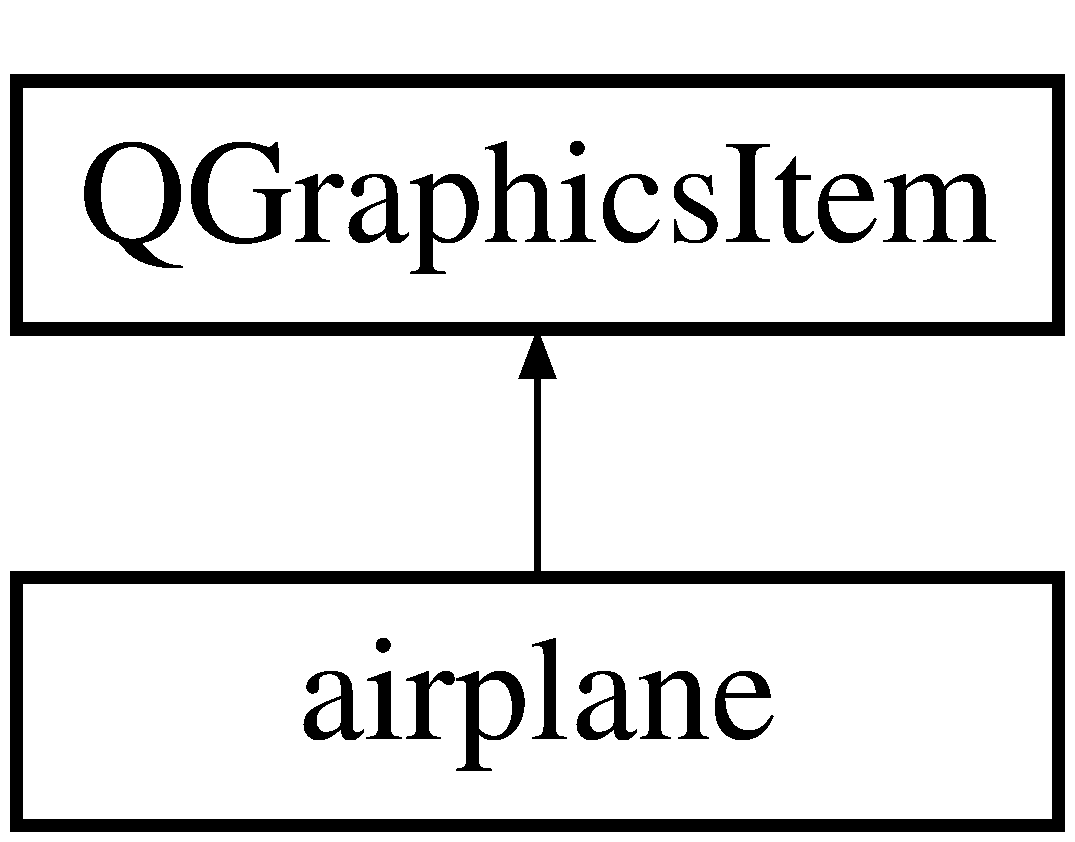
\includegraphics[height=2.000000cm]{classairplane}
\end{center}
\end{figure}
\subsection*{Public Member Functions}
\begin{DoxyCompactItemize}
\item 
\hypertarget{classairplane_a4a004bccf8aecf7d742e0ae486c2a47b}{{\bfseries airplane} (int x, int y, int index, bool direction)}\label{classairplane_a4a004bccf8aecf7d742e0ae486c2a47b}

\end{DoxyCompactItemize}
\subsection*{Protected Member Functions}
\begin{DoxyCompactItemize}
\item 
\hypertarget{classairplane_acaa146bc978062536a9a384c56a8fd5a}{Q\-Rect\-F {\bfseries bounding\-Rect} () const }\label{classairplane_acaa146bc978062536a9a384c56a8fd5a}

\item 
\hypertarget{classairplane_a1f949d8bd0bf33b6368859617845a4c0}{void {\bfseries advance} (int phase)}\label{classairplane_a1f949d8bd0bf33b6368859617845a4c0}

\item 
\hypertarget{classairplane_a48ceb331135cb573b903ebf168f108ac}{void {\bfseries paint} (Q\-Painter $\ast$painter, const Q\-Style\-Option\-Graphics\-Item $\ast$option, Q\-Widget $\ast$widget)}\label{classairplane_a48ceb331135cb573b903ebf168f108ac}

\end{DoxyCompactItemize}
\subsection*{Private Member Functions}
\begin{DoxyCompactItemize}
\item 
\hypertarget{classairplane_ab2059897bc016de2a94544ba431e9d55}{void {\bfseries Do\-Collision} ()}\label{classairplane_ab2059897bc016de2a94544ba431e9d55}

\end{DoxyCompactItemize}
\subsection*{Private Attributes}
\begin{DoxyCompactItemize}
\item 
\hypertarget{classairplane_a5b8f70eba65f453aac157b764a340fef}{qreal {\bfseries starting\-X}}\label{classairplane_a5b8f70eba65f453aac157b764a340fef}

\item 
\hypertarget{classairplane_aa83b58f1d1af21227b2c8f8d7c71f13f}{qreal {\bfseries starting\-Y}}\label{classairplane_aa83b58f1d1af21227b2c8f8d7c71f13f}

\item 
\hypertarget{classairplane_a2bc5817b9956907ad0bf28ac1fdf1d9d}{int {\bfseries airplane\-Index}}\label{classairplane_a2bc5817b9956907ad0bf28ac1fdf1d9d}

\item 
\hypertarget{classairplane_a00664025b42e62b75c42f73025d6efe7}{bool {\bfseries airplane\-Direction}}\label{classairplane_a00664025b42e62b75c42f73025d6efe7}

\item 
\hypertarget{classairplane_a242659249e39d6f4c9dfc7118785724f}{qreal {\bfseries current\-X}}\label{classairplane_a242659249e39d6f4c9dfc7118785724f}

\item 
\hypertarget{classairplane_a1f5fa4aacea7cd4e81e2b881de1e1f4b}{qreal {\bfseries current\-Y}}\label{classairplane_a1f5fa4aacea7cd4e81e2b881de1e1f4b}

\end{DoxyCompactItemize}


The documentation for this class was generated from the following files\-:\begin{DoxyCompactItemize}
\item 
airplane.\-h\item 
airplane.\-cpp\end{DoxyCompactItemize}

\hypertarget{classasteroid}{\section{asteroid Class Reference}
\label{classasteroid}\index{asteroid@{asteroid}}
}
Inheritance diagram for asteroid\-:\begin{figure}[H]
\begin{center}
\leavevmode
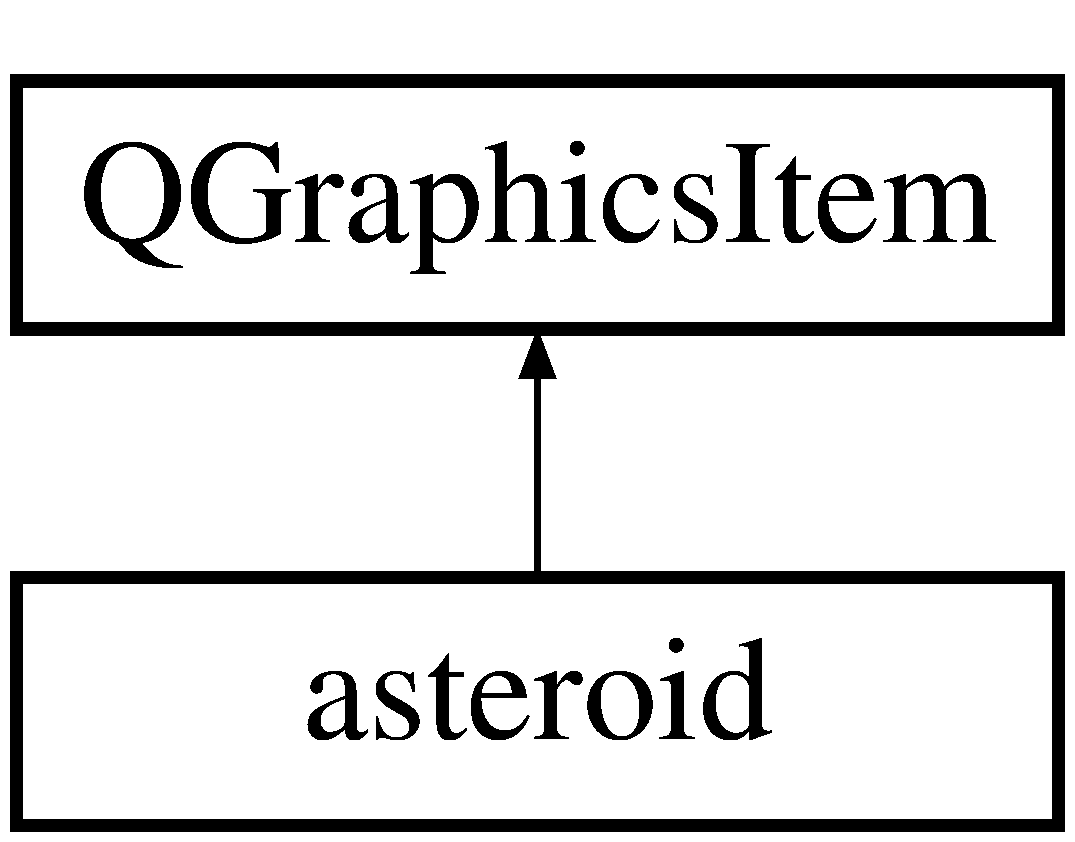
\includegraphics[height=2.000000cm]{classasteroid}
\end{center}
\end{figure}
\subsection*{Public Member Functions}
\begin{DoxyCompactItemize}
\item 
\hyperlink{classasteroid_a7d5c88c543014eb37658e6a45eabe4cb}{asteroid} (int x, int y, int index, bool direction)
\begin{DoxyCompactList}\small\item\em Asteroids fall at diagonal directions and collide with alien. \end{DoxyCompactList}\end{DoxyCompactItemize}
\subsection*{Protected Member Functions}
\begin{DoxyCompactItemize}
\item 
\hypertarget{classasteroid_a9ee6e14e69b3b254b6aa4946dd28ce48}{Q\-Rect\-F {\bfseries bounding\-Rect} () const }\label{classasteroid_a9ee6e14e69b3b254b6aa4946dd28ce48}

\item 
\hypertarget{classasteroid_a09376158d971cab08d4e142c07edddaa}{void {\bfseries advance} (int phase)}\label{classasteroid_a09376158d971cab08d4e142c07edddaa}

\item 
\hypertarget{classasteroid_aa13c3feaa152524d648288e5a775a98e}{void {\bfseries paint} (Q\-Painter $\ast$painter, const Q\-Style\-Option\-Graphics\-Item $\ast$option, Q\-Widget $\ast$widget)}\label{classasteroid_aa13c3feaa152524d648288e5a775a98e}

\end{DoxyCompactItemize}
\subsection*{Private Member Functions}
\begin{DoxyCompactItemize}
\item 
\hypertarget{classasteroid_a63c96ab57771fbcae25bc28b3964de40}{void {\bfseries Do\-Collision} ()}\label{classasteroid_a63c96ab57771fbcae25bc28b3964de40}

\end{DoxyCompactItemize}
\subsection*{Private Attributes}
\begin{DoxyCompactItemize}
\item 
\hypertarget{classasteroid_a3da44e6dbfc556b95e27185cb0f78297}{qreal {\bfseries starting\-X}}\label{classasteroid_a3da44e6dbfc556b95e27185cb0f78297}

\item 
\hypertarget{classasteroid_ad4dab0070eb9556f642fe50f9ada9232}{qreal {\bfseries starting\-Y}}\label{classasteroid_ad4dab0070eb9556f642fe50f9ada9232}

\item 
\hypertarget{classasteroid_a2f7ba0dfccf4fb604feba607feb0daea}{int {\bfseries asteroid\-Index}}\label{classasteroid_a2f7ba0dfccf4fb604feba607feb0daea}

\item 
\hypertarget{classasteroid_a653237a8b60a77e07599ee61533dda0c}{bool {\bfseries asteroid\-Direction}}\label{classasteroid_a653237a8b60a77e07599ee61533dda0c}

\item 
\hypertarget{classasteroid_a642fdd7b78243f43d04f6224ad2bf54c}{qreal {\bfseries asteroid\-Speed}}\label{classasteroid_a642fdd7b78243f43d04f6224ad2bf54c}

\item 
\hypertarget{classasteroid_ac5df03f095024028fb2a61be9695e522}{qreal {\bfseries current\-X}}\label{classasteroid_ac5df03f095024028fb2a61be9695e522}

\item 
\hypertarget{classasteroid_aa0d4082ffca871e9629e45cab1d7c5d2}{qreal {\bfseries current\-Y}}\label{classasteroid_aa0d4082ffca871e9629e45cab1d7c5d2}

\end{DoxyCompactItemize}


\subsection{Constructor \& Destructor Documentation}
\hypertarget{classasteroid_a7d5c88c543014eb37658e6a45eabe4cb}{\index{asteroid@{asteroid}!asteroid@{asteroid}}
\index{asteroid@{asteroid}!asteroid@{asteroid}}
\subsubsection[{asteroid}]{\setlength{\rightskip}{0pt plus 5cm}asteroid\-::asteroid (
\begin{DoxyParamCaption}
\item[{int}]{x, }
\item[{int}]{y, }
\item[{int}]{index, }
\item[{bool}]{direction}
\end{DoxyParamCaption}
)}}\label{classasteroid_a7d5c88c543014eb37658e6a45eabe4cb}


Asteroids fall at diagonal directions and collide with alien. 


\begin{DoxyParams}{Parameters}
{\em x} & starting horizontal position \\
\hline
{\em y} & starting vertical position \\
\hline
{\em index} & numerical index \\
\hline
{\em direction} & direction of travel \\
\hline
\end{DoxyParams}


The documentation for this class was generated from the following files\-:\begin{DoxyCompactItemize}
\item 
asteroid.\-h\item 
asteroid.\-cpp\end{DoxyCompactItemize}

\hypertarget{classastroid}{\section{astroid Class Reference}
\label{classastroid}\index{astroid@{astroid}}
}


The documentation for this class was generated from the following files\-:\begin{DoxyCompactItemize}
\item 
astroid.\-h\item 
astroid.\-cpp\end{DoxyCompactItemize}

\hypertarget{classbackground}{\section{background Class Reference}
\label{classbackground}\index{background@{background}}
}
Inheritance diagram for background\-:\begin{figure}[H]
\begin{center}
\leavevmode
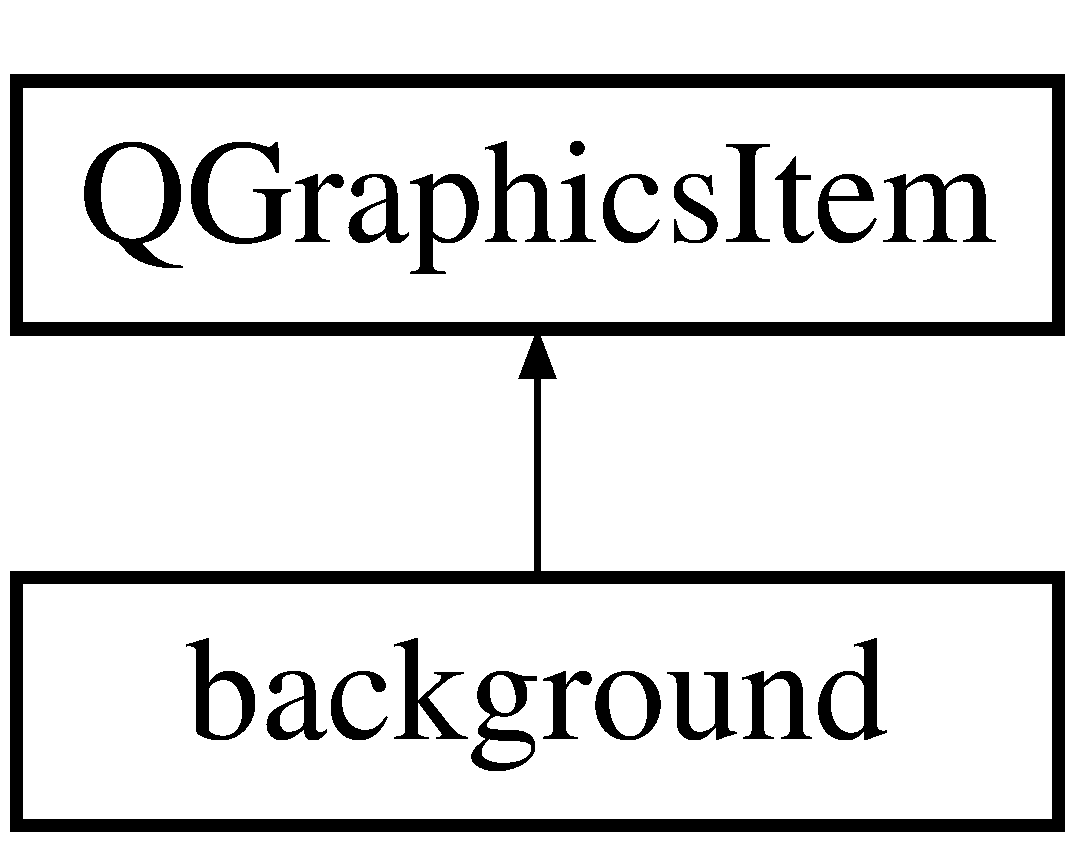
\includegraphics[height=2.000000cm]{classbackground}
\end{center}
\end{figure}
\subsection*{Public Member Functions}
\begin{DoxyCompactItemize}
\item 
\hyperlink{classbackground_a52499a7c34106266039b39b0f9b2dd1b}{background} ()
\item 
\hypertarget{classbackground_aa39a46a96bae7b2ce0d0431253f6845c}{int {\bfseries get\-X} ()}\label{classbackground_aa39a46a96bae7b2ce0d0431253f6845c}

\item 
\hypertarget{classbackground_a6761115f8a866946ae71cf4f06940536}{int {\bfseries get\-Y} ()}\label{classbackground_a6761115f8a866946ae71cf4f06940536}

\end{DoxyCompactItemize}
\subsection*{Public Attributes}
\begin{DoxyCompactItemize}
\item 
\hypertarget{classbackground_ad0fc662cedd9f0858cb2069377767c32}{bool {\bfseries keys\-Pressed} \mbox{[}3\mbox{]}}\label{classbackground_ad0fc662cedd9f0858cb2069377767c32}

\item 
\hypertarget{classbackground_a66fcf6bb73ff645eb3f5260d4893fc53}{bool {\bfseries dead\-Check}}\label{classbackground_a66fcf6bb73ff645eb3f5260d4893fc53}

\item 
\hypertarget{classbackground_a59379ec00d3dd58dbee9dad51e5624c3}{bool {\bfseries dead\-Check2}}\label{classbackground_a59379ec00d3dd58dbee9dad51e5624c3}

\item 
\hypertarget{classbackground_aa1e3d07256205c82aaee71aeee623761}{qreal {\bfseries handling\-Bonus}}\label{classbackground_aa1e3d07256205c82aaee71aeee623761}

\item 
\hypertarget{classbackground_a330368132d6c2a3ca197f692b70b8a09}{qreal {\bfseries strength\-Bonus}}\label{classbackground_a330368132d6c2a3ca197f692b70b8a09}

\item 
\hypertarget{classbackground_acc33d963ba90e9c32fc51debddcd1d73}{qreal {\bfseries current\-X}}\label{classbackground_acc33d963ba90e9c32fc51debddcd1d73}

\item 
\hypertarget{classbackground_a8f4ebdccc996e2326de7520c280db260}{qreal {\bfseries current\-Y}}\label{classbackground_a8f4ebdccc996e2326de7520c280db260}

\item 
\hypertarget{classbackground_ad4d1a3406b730129112e65d0eae546d5}{qreal {\bfseries temp\-\_\-fuel}}\label{classbackground_ad4d1a3406b730129112e65d0eae546d5}

\end{DoxyCompactItemize}
\subsection*{Protected Member Functions}
\begin{DoxyCompactItemize}
\item 
\hypertarget{classbackground_a746278e2456ba524c747b629ce5a084d}{Q\-Rect\-F {\bfseries bounding\-Rect} () const }\label{classbackground_a746278e2456ba524c747b629ce5a084d}

\item 
\hypertarget{classbackground_aaf9de8b66b7715b6373ee83b4ab52f11}{void {\bfseries Do\-Death} ()}\label{classbackground_aaf9de8b66b7715b6373ee83b4ab52f11}

\item 
\hypertarget{classbackground_a920dc4b1432d7b9d00c6637f7c1798b1}{void {\bfseries advance} (int phase)}\label{classbackground_a920dc4b1432d7b9d00c6637f7c1798b1}

\item 
\hypertarget{classbackground_a37489a89173f3e114aef0228245b6e73}{void {\bfseries paint} (Q\-Painter $\ast$painter, const Q\-Style\-Option\-Graphics\-Item $\ast$option, Q\-Widget $\ast$widget)}\label{classbackground_a37489a89173f3e114aef0228245b6e73}

\item 
\hypertarget{classbackground_ae56e6e75013c80f83e8d82789af5ccc7}{virtual void {\bfseries key\-Press\-Event} (Q\-Key\-Event $\ast$event)}\label{classbackground_ae56e6e75013c80f83e8d82789af5ccc7}

\item 
\hypertarget{classbackground_ac09afb24f88ccc2c1878a282d01c16a1}{virtual void {\bfseries key\-Release\-Event} (Q\-Key\-Event $\ast$event)}\label{classbackground_ac09afb24f88ccc2c1878a282d01c16a1}

\end{DoxyCompactItemize}
\subsection*{Private Attributes}
\begin{DoxyCompactItemize}
\item 
\hypertarget{classbackground_a81b5ffc16339465f94e0f7ee47f84e7c}{Q\-String {\bfseries str\-\_\-mins}}\label{classbackground_a81b5ffc16339465f94e0f7ee47f84e7c}

\item 
\hypertarget{classbackground_a9e0e1509f02aa5da66710736665885d0}{Q\-String {\bfseries str\-\_\-fuel}}\label{classbackground_a9e0e1509f02aa5da66710736665885d0}

\item 
\hypertarget{classbackground_a324ba07a8a40473878b7f0d282214342}{Q\-String {\bfseries str\-\_\-lives}}\label{classbackground_a324ba07a8a40473878b7f0d282214342}

\end{DoxyCompactItemize}


\subsection{Constructor \& Destructor Documentation}
\hypertarget{classbackground_a52499a7c34106266039b39b0f9b2dd1b}{\index{background@{background}!background@{background}}
\index{background@{background}!background@{background}}
\subsubsection[{background}]{\setlength{\rightskip}{0pt plus 5cm}background\-::background (
\begin{DoxyParamCaption}
{}
\end{DoxyParamCaption}
)}}\label{classbackground_a52499a7c34106266039b39b0f9b2dd1b}

\begin{DoxyParams}{Parameters}
{\em x} & this is a sweet parameter \\
\hline
{\em y} & waoh coolio\-This class governs all physics control The \char`\"{}background\char`\"{} moves depending on the global\-X and global\-Y variables This simulates movement of the alien Updates of game text are used in this class Checks for death and other attributes are given \\
\hline
\end{DoxyParams}


The documentation for this class was generated from the following files\-:\begin{DoxyCompactItemize}
\item 
background.\-h\item 
background.\-cpp\end{DoxyCompactItemize}

\hypertarget{classbackground2}{\section{background2 Class Reference}
\label{classbackground2}\index{background2@{background2}}
}
Inheritance diagram for background2\-:\begin{figure}[H]
\begin{center}
\leavevmode
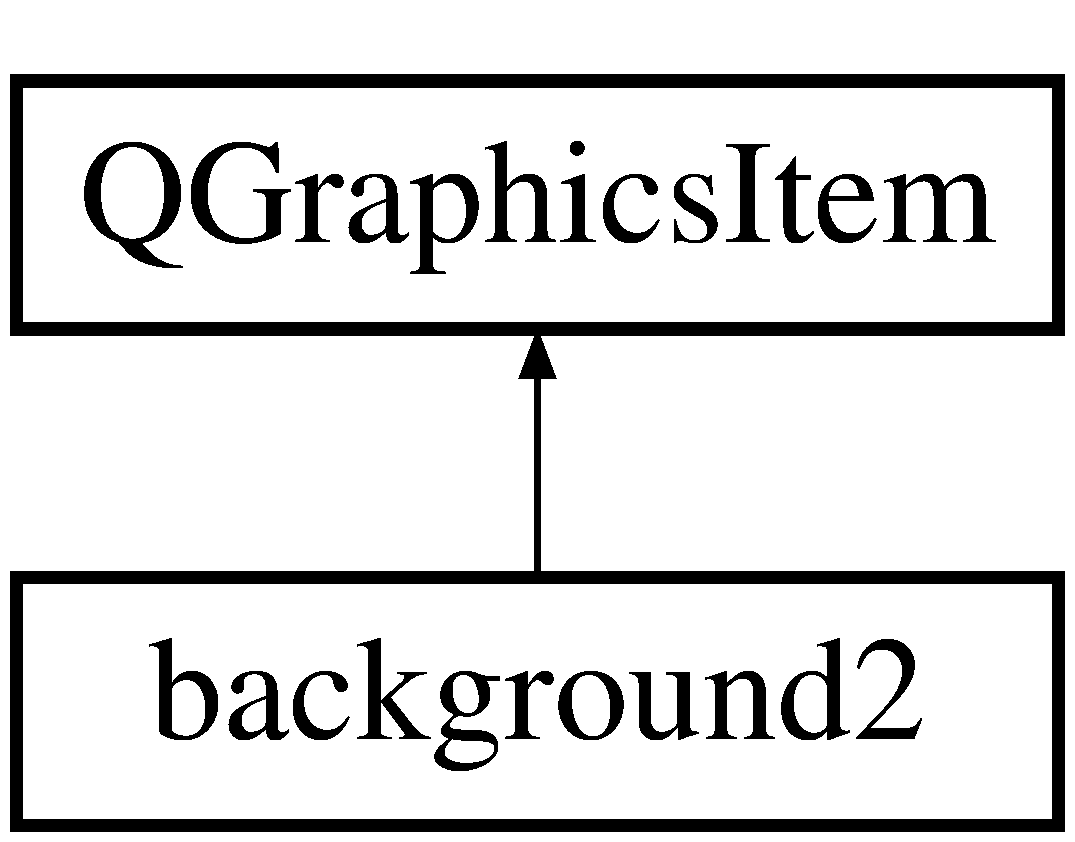
\includegraphics[height=2.000000cm]{classbackground2}
\end{center}
\end{figure}
\subsection*{Public Member Functions}
\begin{DoxyCompactItemize}
\item 
\hypertarget{classbackground2_a268ee2f21e35112e47a8dd6c287f82cb}{\hyperlink{classbackground2_a268ee2f21e35112e47a8dd6c287f82cb}{background2} ()}\label{classbackground2_a268ee2f21e35112e47a8dd6c287f82cb}

\begin{DoxyCompactList}\small\item\em This is an additional layer of sky above the first. \end{DoxyCompactList}\end{DoxyCompactItemize}
\subsection*{Protected Member Functions}
\begin{DoxyCompactItemize}
\item 
\hypertarget{classbackground2_a8d1e5049e4589879d20fbee704074c60}{Q\-Rect\-F {\bfseries bounding\-Rect} () const }\label{classbackground2_a8d1e5049e4589879d20fbee704074c60}

\item 
\hypertarget{classbackground2_ae9c85e5b171bb6ead3497e8e535d120f}{void {\bfseries paint} (Q\-Painter $\ast$painter, const Q\-Style\-Option\-Graphics\-Item $\ast$option, Q\-Widget $\ast$widget)}\label{classbackground2_ae9c85e5b171bb6ead3497e8e535d120f}

\end{DoxyCompactItemize}


The documentation for this class was generated from the following files\-:\begin{DoxyCompactItemize}
\item 
background2.\-h\item 
background2.\-cpp\end{DoxyCompactItemize}

\hypertarget{classbackground3}{\section{background3 Class Reference}
\label{classbackground3}\index{background3@{background3}}
}
Inheritance diagram for background3\-:\begin{figure}[H]
\begin{center}
\leavevmode
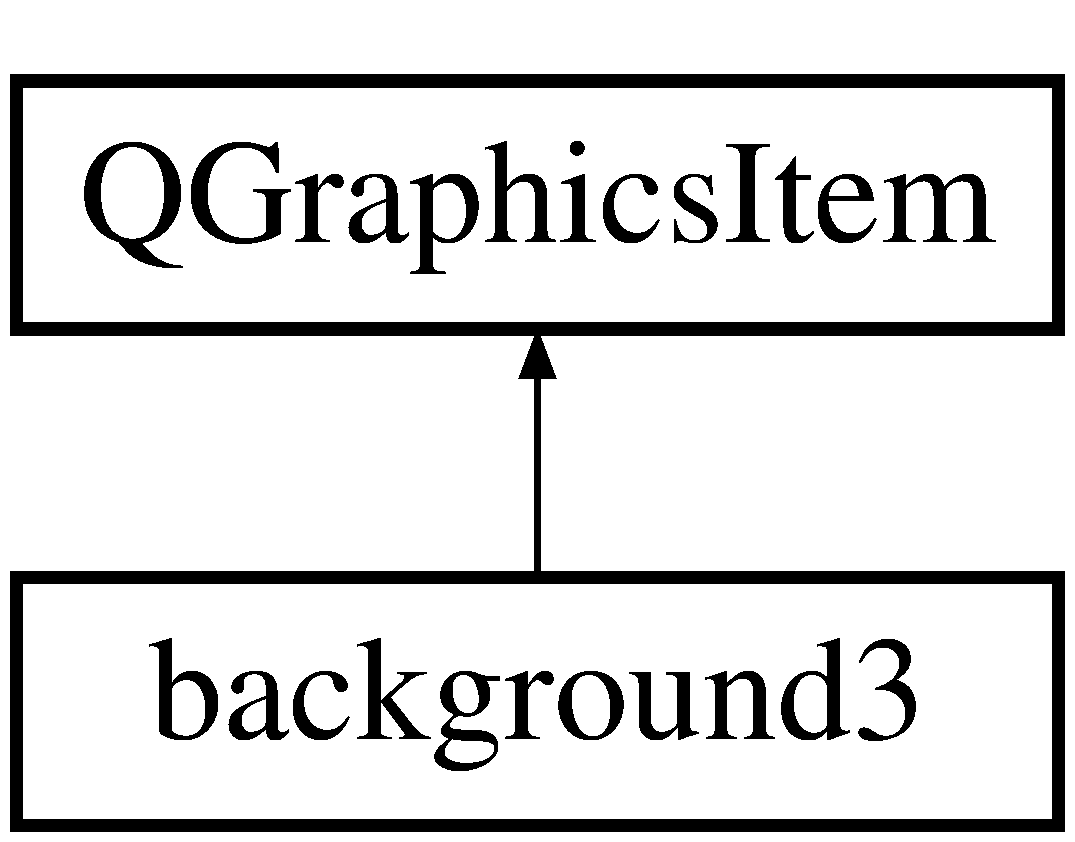
\includegraphics[height=2.000000cm]{classbackground3}
\end{center}
\end{figure}
\subsection*{Public Member Functions}
\begin{DoxyCompactItemize}
\item 
\hypertarget{classbackground3_a742028d653682b5e7227967f84f8025b}{\hyperlink{classbackground3_a742028d653682b5e7227967f84f8025b}{background3} ()}\label{classbackground3_a742028d653682b5e7227967f84f8025b}

\begin{DoxyCompactList}\small\item\em This represents outer space within the game. \end{DoxyCompactList}\end{DoxyCompactItemize}
\subsection*{Protected Member Functions}
\begin{DoxyCompactItemize}
\item 
\hypertarget{classbackground3_a6dad89c5a92e1564e36bdf6e795d725f}{Q\-Rect\-F {\bfseries bounding\-Rect} () const }\label{classbackground3_a6dad89c5a92e1564e36bdf6e795d725f}

\item 
\hypertarget{classbackground3_ab17c347405b194fb860d0f036e78f22d}{void {\bfseries paint} (Q\-Painter $\ast$painter, const Q\-Style\-Option\-Graphics\-Item $\ast$option, Q\-Widget $\ast$widget)}\label{classbackground3_ab17c347405b194fb860d0f036e78f22d}

\end{DoxyCompactItemize}


The documentation for this class was generated from the following files\-:\begin{DoxyCompactItemize}
\item 
background3.\-h\item 
background3.\-cpp\end{DoxyCompactItemize}

\hypertarget{classbird}{\section{bird Class Reference}
\label{classbird}\index{bird@{bird}}
}
Inheritance diagram for bird\-:\begin{figure}[H]
\begin{center}
\leavevmode
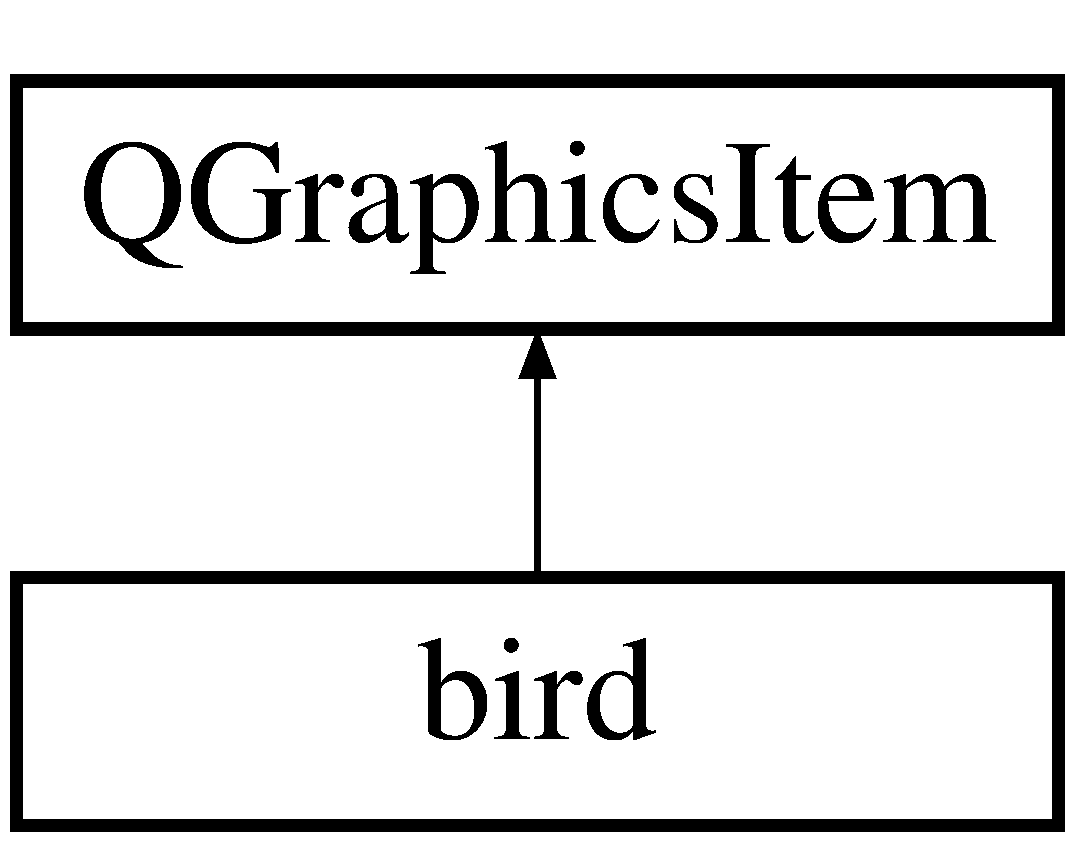
\includegraphics[height=2.000000cm]{classbird}
\end{center}
\end{figure}
\subsection*{Public Member Functions}
\begin{DoxyCompactItemize}
\item 
\hyperlink{classbird_a140b91610200bc6580693c3aae7a362b}{bird} (int x, int y, int index, bool direction)
\begin{DoxyCompactList}\small\item\em Birds fly across the screen and collide with the alien. \end{DoxyCompactList}\end{DoxyCompactItemize}
\subsection*{Protected Member Functions}
\begin{DoxyCompactItemize}
\item 
\hypertarget{classbird_a237e6ad81998aeaf1be45bcb1e04dc7f}{Q\-Rect\-F {\bfseries bounding\-Rect} () const }\label{classbird_a237e6ad81998aeaf1be45bcb1e04dc7f}

\item 
\hypertarget{classbird_ac3888e6dad82bdff34cb6219b474fcb1}{void {\bfseries advance} (int phase)}\label{classbird_ac3888e6dad82bdff34cb6219b474fcb1}

\item 
\hypertarget{classbird_adfe0751f94a46ac337161af3f5fe6a66}{void {\bfseries paint} (Q\-Painter $\ast$painter, const Q\-Style\-Option\-Graphics\-Item $\ast$option, Q\-Widget $\ast$widget)}\label{classbird_adfe0751f94a46ac337161af3f5fe6a66}

\end{DoxyCompactItemize}
\subsection*{Private Member Functions}
\begin{DoxyCompactItemize}
\item 
\hypertarget{classbird_af879cd57331fed816b31c9c55dccc2d3}{void {\bfseries Do\-Collision} ()}\label{classbird_af879cd57331fed816b31c9c55dccc2d3}

\end{DoxyCompactItemize}
\subsection*{Private Attributes}
\begin{DoxyCompactItemize}
\item 
\hypertarget{classbird_af7b5a9bd3d6b251b619f40f8b0b9f9c2}{qreal {\bfseries starting\-X}}\label{classbird_af7b5a9bd3d6b251b619f40f8b0b9f9c2}

\item 
\hypertarget{classbird_ae2fa3b28fa9cc254ab5bba8a059ce21e}{qreal {\bfseries starting\-Y}}\label{classbird_ae2fa3b28fa9cc254ab5bba8a059ce21e}

\item 
\hypertarget{classbird_a76b8b717e08d5ca53362bf2d51ce5129}{int {\bfseries bird\-Index}}\label{classbird_a76b8b717e08d5ca53362bf2d51ce5129}

\item 
\hypertarget{classbird_aec894456d4a79babbe8ec0fcec89bde9}{bool {\bfseries bird\-Direction}}\label{classbird_aec894456d4a79babbe8ec0fcec89bde9}

\item 
\hypertarget{classbird_a8f35516c51ff45a4b0e871f55a31f023}{qreal {\bfseries current\-X}}\label{classbird_a8f35516c51ff45a4b0e871f55a31f023}

\item 
\hypertarget{classbird_a1b350aac1f8b5784818d4cd298394385}{qreal {\bfseries current\-Y}}\label{classbird_a1b350aac1f8b5784818d4cd298394385}

\item 
\hypertarget{classbird_a467e826c1b91d9271a8225e2f63b8be4}{qreal {\bfseries bird\-Speed}}\label{classbird_a467e826c1b91d9271a8225e2f63b8be4}

\end{DoxyCompactItemize}


\subsection{Constructor \& Destructor Documentation}
\hypertarget{classbird_a140b91610200bc6580693c3aae7a362b}{\index{bird@{bird}!bird@{bird}}
\index{bird@{bird}!bird@{bird}}
\subsubsection[{bird}]{\setlength{\rightskip}{0pt plus 5cm}bird\-::bird (
\begin{DoxyParamCaption}
\item[{int}]{x, }
\item[{int}]{y, }
\item[{int}]{index, }
\item[{bool}]{direction}
\end{DoxyParamCaption}
)}}\label{classbird_a140b91610200bc6580693c3aae7a362b}


Birds fly across the screen and collide with the alien. 


\begin{DoxyParams}{Parameters}
{\em x} & starting horizontal position \\
\hline
{\em y} & starting vertical position \\
\hline
{\em index} & numerical index \\
\hline
{\em direction} & direction of travel \\
\hline
\end{DoxyParams}


The documentation for this class was generated from the following files\-:\begin{DoxyCompactItemize}
\item 
bird.\-h\item 
bird.\-cpp\end{DoxyCompactItemize}

\hypertarget{classblackout}{\section{blackout Class Reference}
\label{classblackout}\index{blackout@{blackout}}
}
Inheritance diagram for blackout\-:\begin{figure}[H]
\begin{center}
\leavevmode
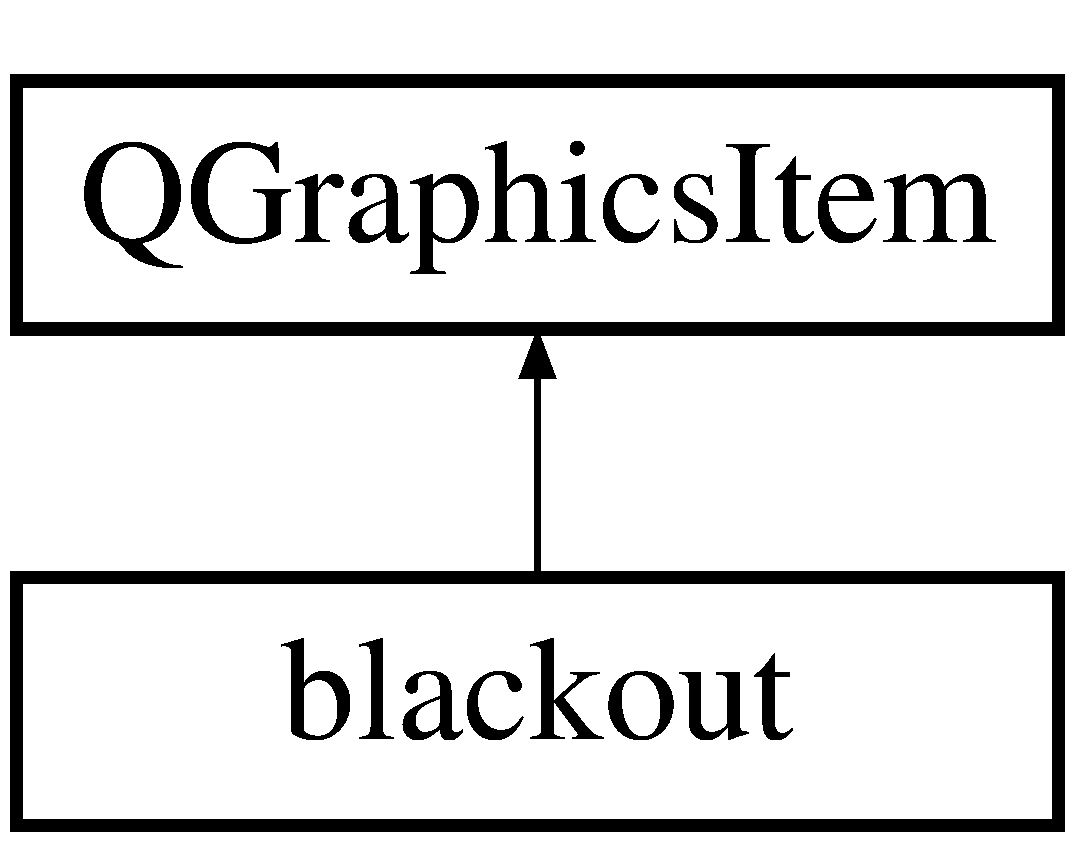
\includegraphics[height=2.000000cm]{classblackout}
\end{center}
\end{figure}
\subsection*{Public Member Functions}
\begin{DoxyCompactItemize}
\item 
\hyperlink{classblackout_a1e8c7f06ebea0ab98c2ea0aab0c72300}{blackout} (int x, int y, int index, bool direction)
\begin{DoxyCompactList}\small\item\em The blackout displays a black image over everything, disrupting play. \end{DoxyCompactList}\item 
\hypertarget{classblackout_aff541e3caaa1ba4db81bde5d5e822fe7}{void {\bfseries respawn} ()}\label{classblackout_aff541e3caaa1ba4db81bde5d5e822fe7}

\end{DoxyCompactItemize}
\subsection*{Protected Member Functions}
\begin{DoxyCompactItemize}
\item 
\hypertarget{classblackout_af5d2e60c2b84a2669b32f6a4c6db568f}{Q\-Rect\-F {\bfseries bounding\-Rect} () const }\label{classblackout_af5d2e60c2b84a2669b32f6a4c6db568f}

\item 
\hypertarget{classblackout_a4fd80f944889504df0f257cae59a3e80}{void {\bfseries advance} (int phase)}\label{classblackout_a4fd80f944889504df0f257cae59a3e80}

\item 
\hypertarget{classblackout_a5e22133a5308e7a4cbeeff58a8a87547}{void {\bfseries paint} (Q\-Painter $\ast$painter, const Q\-Style\-Option\-Graphics\-Item $\ast$option, Q\-Widget $\ast$widget)}\label{classblackout_a5e22133a5308e7a4cbeeff58a8a87547}

\end{DoxyCompactItemize}
\subsection*{Private Member Functions}
\begin{DoxyCompactItemize}
\item 
\hypertarget{classblackout_a68dda60fb533ec6e578c59790899e4b5}{void {\bfseries Do\-Collision} ()}\label{classblackout_a68dda60fb533ec6e578c59790899e4b5}

\end{DoxyCompactItemize}
\subsection*{Private Attributes}
\begin{DoxyCompactItemize}
\item 
\hypertarget{classblackout_a3ae61ab41918803a9d9c27d088829c01}{qreal {\bfseries starting\-X}}\label{classblackout_a3ae61ab41918803a9d9c27d088829c01}

\item 
\hypertarget{classblackout_a275734a6921bbba7880ebda0c20c436f}{qreal {\bfseries starting\-Y}}\label{classblackout_a275734a6921bbba7880ebda0c20c436f}

\item 
\hypertarget{classblackout_a80a12abbc15307e3cc92e20a7617ee87}{int {\bfseries blackout\-Index}}\label{classblackout_a80a12abbc15307e3cc92e20a7617ee87}

\item 
\hypertarget{classblackout_a53173b60d6f11714847898136c034471}{bool {\bfseries blackout\-Direction}}\label{classblackout_a53173b60d6f11714847898136c034471}

\item 
\hypertarget{classblackout_af005db656ad9129781a740837c12b444}{qreal {\bfseries blackout\-Speed}}\label{classblackout_af005db656ad9129781a740837c12b444}

\item 
\hypertarget{classblackout_a4706fbdcacf06793117040b0e85a3f18}{qreal {\bfseries current\-X}}\label{classblackout_a4706fbdcacf06793117040b0e85a3f18}

\item 
\hypertarget{classblackout_a9269902c8ea235ff4e5c003dfac3c901}{qreal {\bfseries current\-Y}}\label{classblackout_a9269902c8ea235ff4e5c003dfac3c901}

\end{DoxyCompactItemize}


\subsection{Constructor \& Destructor Documentation}
\hypertarget{classblackout_a1e8c7f06ebea0ab98c2ea0aab0c72300}{\index{blackout@{blackout}!blackout@{blackout}}
\index{blackout@{blackout}!blackout@{blackout}}
\subsubsection[{blackout}]{\setlength{\rightskip}{0pt plus 5cm}blackout\-::blackout (
\begin{DoxyParamCaption}
\item[{int}]{x, }
\item[{int}]{y, }
\item[{int}]{index, }
\item[{bool}]{direction}
\end{DoxyParamCaption}
)}}\label{classblackout_a1e8c7f06ebea0ab98c2ea0aab0c72300}


The blackout displays a black image over everything, disrupting play. 


\begin{DoxyParams}{Parameters}
{\em x} & starting horizontal position \\
\hline
{\em y} & starting vertical position \\
\hline
{\em index} & numerical index \\
\hline
{\em direction} & direction of travel \\
\hline
\end{DoxyParams}


The documentation for this class was generated from the following files\-:\begin{DoxyCompactItemize}
\item 
blackout.\-h\item 
blackout.\-cpp\end{DoxyCompactItemize}

\hypertarget{class_dialog}{\section{Dialog Class Reference}
\label{class_dialog}\index{Dialog@{Dialog}}
}
Inheritance diagram for Dialog\-:\begin{figure}[H]
\begin{center}
\leavevmode
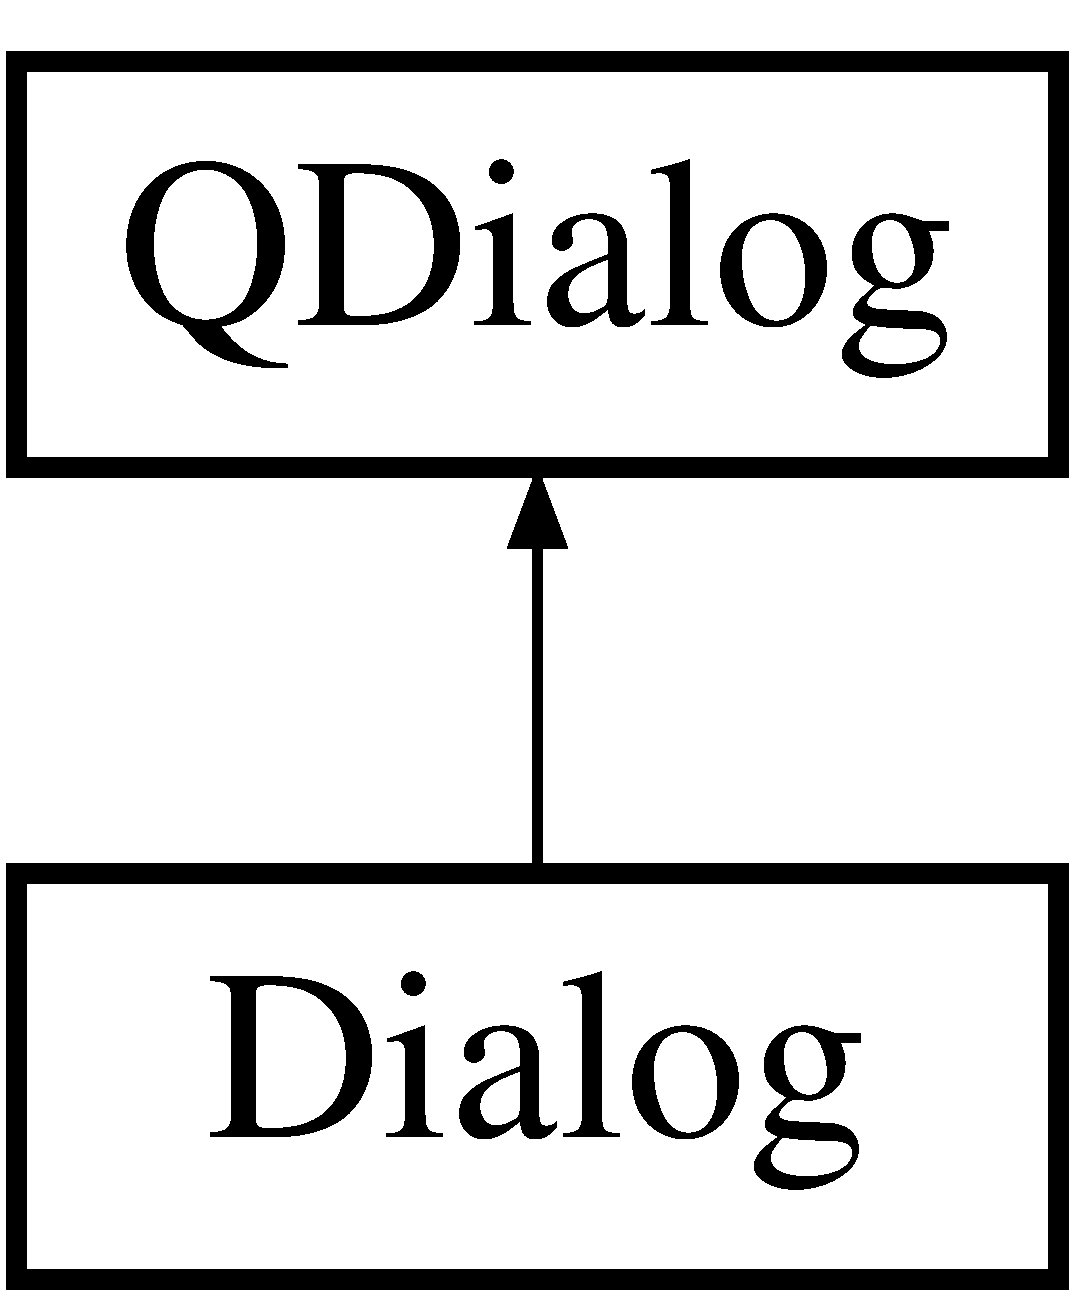
\includegraphics[height=2.000000cm]{class_dialog}
\end{center}
\end{figure}
\subsection*{Public Member Functions}
\begin{DoxyCompactItemize}
\item 
\hypertarget{class_dialog_acfa2063f9f962d394c6a645b6e7e08d8}{{\bfseries Dialog} (Q\-Widget $\ast$parent=0)}\label{class_dialog_acfa2063f9f962d394c6a645b6e7e08d8}

\end{DoxyCompactItemize}
\subsection*{Public Attributes}
\begin{DoxyCompactItemize}
\item 
\hypertarget{class_dialog_aaa4b5bfb9a0f64900d524f14bc32e6df}{Ui\-::\-Dialog $\ast$ {\bfseries ui}}\label{class_dialog_aaa4b5bfb9a0f64900d524f14bc32e6df}

\item 
\hypertarget{class_dialog_a2e726c6a62fa7cf2cec0d2a555b54593}{Q\-Graphics\-Scene $\ast$ {\bfseries scene}}\label{class_dialog_a2e726c6a62fa7cf2cec0d2a555b54593}

\item 
\hypertarget{class_dialog_a87becbd8566b731be26fbf8af7a02e00}{Q\-Graphics\-Scene $\ast$ {\bfseries scene\-Shop}}\label{class_dialog_a87becbd8566b731be26fbf8af7a02e00}

\item 
\hypertarget{class_dialog_a318f75a00c958a671a8306ce27dc4cbb}{Q\-Graphics\-Scene $\ast$ {\bfseries scene\-Menu}}\label{class_dialog_a318f75a00c958a671a8306ce27dc4cbb}

\item 
\hypertarget{class_dialog_a321fa4c0b6026f8ba8ae45b25ae6c5dc}{Q\-Graphics\-Scene $\ast$ {\bfseries scene\-Instruction}}\label{class_dialog_a321fa4c0b6026f8ba8ae45b25ae6c5dc}

\item 
\hypertarget{class_dialog_a1831f616ec83e8d5a3c1255e0a091c65}{Q\-Graphics\-Scene $\ast$ {\bfseries scene\-Script}}\label{class_dialog_a1831f616ec83e8d5a3c1255e0a091c65}

\end{DoxyCompactItemize}
\subsection*{Protected Member Functions}
\begin{DoxyCompactItemize}
\item 
\hypertarget{class_dialog_a57bbf55fbef632d7f36c30be1dbb0967}{void {\bfseries paint} (Q\-Painter $\ast$painter, const Q\-Style\-Option\-Graphics\-Item $\ast$option, Q\-Widget $\ast$widget)}\label{class_dialog_a57bbf55fbef632d7f36c30be1dbb0967}

\end{DoxyCompactItemize}
\subsection*{Private Slots}
\begin{DoxyCompactItemize}
\item 
\hypertarget{class_dialog_a98d5e2a625602be0bb710b8ac2ff19a3}{void \hyperlink{class_dialog_a98d5e2a625602be0bb710b8ac2ff19a3}{game\-Next\-Scene} ()}\label{class_dialog_a98d5e2a625602be0bb710b8ac2ff19a3}

\begin{DoxyCompactList}\small\item\em Goes to shop. \end{DoxyCompactList}\item 
\hypertarget{class_dialog_a5db671e5182ffdcc2459489068b09e35}{void \hyperlink{class_dialog_a5db671e5182ffdcc2459489068b09e35}{shop\-Next\-Scene} ()}\label{class_dialog_a5db671e5182ffdcc2459489068b09e35}

\begin{DoxyCompactList}\small\item\em starts new day \end{DoxyCompactList}\item 
\hypertarget{class_dialog_a90f373cdb54057625ae6d84dc44ee03e}{void \hyperlink{class_dialog_a90f373cdb54057625ae6d84dc44ee03e}{day\-Start} ()}\label{class_dialog_a90f373cdb54057625ae6d84dc44ee03e}

\begin{DoxyCompactList}\small\item\em start of day text \end{DoxyCompactList}\item 
\hypertarget{class_dialog_a1e35ca10fa299339816ff36590526496}{void \hyperlink{class_dialog_a1e35ca10fa299339816ff36590526496}{on\-\_\-play\-Button\-\_\-clicked} ()}\label{class_dialog_a1e35ca10fa299339816ff36590526496}

\begin{DoxyCompactList}\small\item\em when play is pushed \end{DoxyCompactList}\item 
\hypertarget{class_dialog_a25f811678b39e8375ea5bc0df6063a9a}{void \hyperlink{class_dialog_a25f811678b39e8375ea5bc0df6063a9a}{on\-\_\-instructions\-Button\-\_\-clicked} ()}\label{class_dialog_a25f811678b39e8375ea5bc0df6063a9a}

\begin{DoxyCompactList}\small\item\em when instructions is pushed \end{DoxyCompactList}\item 
\hypertarget{class_dialog_a27969c9386dbad7fc98adb235c143e7b}{void \hyperlink{class_dialog_a27969c9386dbad7fc98adb235c143e7b}{on\-\_\-exit\-Button\-\_\-clicked} ()}\label{class_dialog_a27969c9386dbad7fc98adb235c143e7b}

\begin{DoxyCompactList}\small\item\em when exit is pushed \end{DoxyCompactList}\item 
\hypertarget{class_dialog_a5e6ec65f6732629ca8a8433fd182e73a}{void \hyperlink{class_dialog_a5e6ec65f6732629ca8a8433fd182e73a}{on\-\_\-play\-Button2\-\_\-clicked} ()}\label{class_dialog_a5e6ec65f6732629ca8a8433fd182e73a}

\begin{DoxyCompactList}\small\item\em when playbutton2 is pushed \end{DoxyCompactList}\item 
\hypertarget{class_dialog_ac2a85847a1a1d608d9736a65e4a58406}{void \hyperlink{class_dialog_ac2a85847a1a1d608d9736a65e4a58406}{on\-\_\-menu\-Button\-\_\-clicked} ()}\label{class_dialog_ac2a85847a1a1d608d9736a65e4a58406}

\begin{DoxyCompactList}\small\item\em when menu is pushed \end{DoxyCompactList}\item 
\hypertarget{class_dialog_a485961309d5073b5affe91419f9848ef}{void \hyperlink{class_dialog_a485961309d5073b5affe91419f9848ef}{on\-\_\-exit\-Button2\-\_\-clicked} ()}\label{class_dialog_a485961309d5073b5affe91419f9848ef}

\begin{DoxyCompactList}\small\item\em when exitbutton2 is pushed \end{DoxyCompactList}\item 
\hypertarget{class_dialog_aba2e6cbe0699f726c2cd3415c20684ee}{void \hyperlink{class_dialog_aba2e6cbe0699f726c2cd3415c20684ee}{blackout\-Done} ()}\label{class_dialog_aba2e6cbe0699f726c2cd3415c20684ee}

\begin{DoxyCompactList}\small\item\em when blackout is done \end{DoxyCompactList}\item 
\hypertarget{class_dialog_a5e653743b5e3ec76e987c4255ab01865}{void \hyperlink{class_dialog_a5e653743b5e3ec76e987c4255ab01865}{dark\-Done} ()}\label{class_dialog_a5e653743b5e3ec76e987c4255ab01865}

\begin{DoxyCompactList}\small\item\em residual effect of blackout \end{DoxyCompactList}\item 
\hypertarget{class_dialog_a3631980bb77b7deb3bd2aceee3776605}{void \hyperlink{class_dialog_a3631980bb77b7deb3bd2aceee3776605}{pet\-Done} ()}\label{class_dialog_a3631980bb77b7deb3bd2aceee3776605}

\begin{DoxyCompactList}\small\item\em no more pet invulnerability/speed \end{DoxyCompactList}\end{DoxyCompactItemize}
\subsection*{Private Attributes}
\begin{DoxyCompactItemize}
\item 
\hypertarget{class_dialog_a6d45d7fc1a2c6918f56863c4a746efde}{Q\-String {\bfseries str}}\label{class_dialog_a6d45d7fc1a2c6918f56863c4a746efde}

\item 
\hypertarget{class_dialog_a1068edc205b39df0b43962b67cd343ea}{Q\-Sound $\ast$ {\bfseries sound}}\label{class_dialog_a1068edc205b39df0b43962b67cd343ea}

\item 
\hypertarget{class_dialog_a75dc0bd381c7a9bcae106774b6afc21b}{Q\-Sound $\ast$ {\bfseries sound2}}\label{class_dialog_a75dc0bd381c7a9bcae106774b6afc21b}

\item 
\hypertarget{class_dialog_aa315cc7ff54f0d024bf6fdb3cd10b4eb}{\hyperlink{classplane}{plane} $\ast$ {\bfseries plane\-\_\-1}}\label{class_dialog_aa315cc7ff54f0d024bf6fdb3cd10b4eb}

\item 
\hypertarget{class_dialog_acc37ed0151510374d48655ad9997e811}{\hyperlink{classplane}{plane} $\ast$ {\bfseries plane\-\_\-2}}\label{class_dialog_acc37ed0151510374d48655ad9997e811}

\item 
\hypertarget{class_dialog_a82db7cfbde0c925e426d470388a12a89}{\hyperlink{classplane}{plane} $\ast$ {\bfseries plane\-\_\-3}}\label{class_dialog_a82db7cfbde0c925e426d470388a12a89}

\item 
\hypertarget{class_dialog_a64338e2582ef62300e5a53474114cf98}{\hyperlink{classplane}{plane} $\ast$ {\bfseries plane\-\_\-4}}\label{class_dialog_a64338e2582ef62300e5a53474114cf98}

\item 
\hypertarget{class_dialog_ad689b8dffe4cca4c7353e2141bc6b62b}{\hyperlink{classplane}{plane} $\ast$ {\bfseries plane\-\_\-5}}\label{class_dialog_ad689b8dffe4cca4c7353e2141bc6b62b}

\item 
\hypertarget{class_dialog_ae53c7d42ca9be327da18a568bf2b3343}{\hyperlink{classplane}{plane} $\ast$ {\bfseries plane\-\_\-6}}\label{class_dialog_ae53c7d42ca9be327da18a568bf2b3343}

\item 
\hypertarget{class_dialog_a1c932eee6c1c506c969550357c2bcc75}{\hyperlink{classplane}{plane} $\ast$ {\bfseries plane\-\_\-7}}\label{class_dialog_a1c932eee6c1c506c969550357c2bcc75}

\item 
\hypertarget{class_dialog_acdc7cc5585061fde0c72880d09757290}{\hyperlink{classplane}{plane} $\ast$ {\bfseries plane\-\_\-8}}\label{class_dialog_acdc7cc5585061fde0c72880d09757290}

\item 
\hypertarget{class_dialog_a205685f973d4c0ca0f08ead59b853a06}{\hyperlink{classplane}{plane} $\ast$ {\bfseries plane\-\_\-9}}\label{class_dialog_a205685f973d4c0ca0f08ead59b853a06}

\item 
\hypertarget{class_dialog_aba4b1e560ad228c86862c41f83869c38}{\hyperlink{classplane}{plane} $\ast$ {\bfseries plane\-\_\-10}}\label{class_dialog_aba4b1e560ad228c86862c41f83869c38}

\item 
\hypertarget{class_dialog_a68d812fcdd5ee7867beabf730e763d4e}{\hyperlink{classplane}{plane} $\ast$ {\bfseries plane\-\_\-11}}\label{class_dialog_a68d812fcdd5ee7867beabf730e763d4e}

\item 
\hypertarget{class_dialog_a3b3f2a1f81de7765b8bceb2e0873caf5}{\hyperlink{classplane}{plane} $\ast$ {\bfseries plane\-\_\-12}}\label{class_dialog_a3b3f2a1f81de7765b8bceb2e0873caf5}

\item 
\hypertarget{class_dialog_adf00f9d84331a64b1bf5fe6b8e8145c2}{\hyperlink{classplane}{plane} $\ast$ {\bfseries plane\-\_\-13}}\label{class_dialog_adf00f9d84331a64b1bf5fe6b8e8145c2}

\item 
\hypertarget{class_dialog_a4789bb9033975a51a24979cdb901bc32}{\hyperlink{classplane}{plane} $\ast$ {\bfseries plane\-\_\-14}}\label{class_dialog_a4789bb9033975a51a24979cdb901bc32}

\item 
\hypertarget{class_dialog_ac1421f894b808d9ef1fd7049297e829c}{\hyperlink{classplane}{plane} $\ast$ {\bfseries plane\-\_\-15}}\label{class_dialog_ac1421f894b808d9ef1fd7049297e829c}

\item 
\hypertarget{class_dialog_a3accb453fbbf3e62cd0d1182f89556ba}{\hyperlink{classplane}{plane} $\ast$ {\bfseries plane\-\_\-16}}\label{class_dialog_a3accb453fbbf3e62cd0d1182f89556ba}

\item 
\hypertarget{class_dialog_ab76c055a6e7513142f8eb7f0c672006f}{\hyperlink{classplane}{plane} $\ast$ {\bfseries plane\-\_\-17}}\label{class_dialog_ab76c055a6e7513142f8eb7f0c672006f}

\item 
\hypertarget{class_dialog_a956bd661f7083583c599905e0657d91c}{\hyperlink{classplane}{plane} $\ast$ {\bfseries plane\-\_\-18}}\label{class_dialog_a956bd661f7083583c599905e0657d91c}

\item 
\hypertarget{class_dialog_a88f0db334106d92ba2ab152e51e88685}{\hyperlink{classplane}{plane} $\ast$ {\bfseries plane\-\_\-19}}\label{class_dialog_a88f0db334106d92ba2ab152e51e88685}

\item 
\hypertarget{class_dialog_ae9e58d898e3fab0574b237726df1fa08}{\hyperlink{classplane}{plane} $\ast$ {\bfseries plane\-\_\-20}}\label{class_dialog_ae9e58d898e3fab0574b237726df1fa08}

\item 
\hypertarget{class_dialog_a53bf5349057ff58acf908fa24bbd027a}{\hyperlink{classplane}{plane} $\ast$ {\bfseries plane\-\_\-21}}\label{class_dialog_a53bf5349057ff58acf908fa24bbd027a}

\item 
\hypertarget{class_dialog_a898f04d62b93ed6eb7982c4f8c558ee7}{\hyperlink{classplane}{plane} $\ast$ {\bfseries plane\-\_\-22}}\label{class_dialog_a898f04d62b93ed6eb7982c4f8c558ee7}

\item 
\hypertarget{class_dialog_afa028e50dd2ad2a08b585a29e4a7db10}{\hyperlink{classplane}{plane} $\ast$ {\bfseries plane\-\_\-23}}\label{class_dialog_afa028e50dd2ad2a08b585a29e4a7db10}

\item 
\hypertarget{class_dialog_a9ca0f2c504dbb31d0c43efc4a5f88510}{\hyperlink{classplane}{plane} $\ast$ {\bfseries plane\-\_\-24}}\label{class_dialog_a9ca0f2c504dbb31d0c43efc4a5f88510}

\item 
\hypertarget{class_dialog_a95729a0c17a644890a2e35f119a3bc68}{\hyperlink{classbird}{bird} $\ast$ {\bfseries bird\-\_\-1}}\label{class_dialog_a95729a0c17a644890a2e35f119a3bc68}

\item 
\hypertarget{class_dialog_a4eb01fd78e09c7747fc39f67cf03b28f}{\hyperlink{classbird}{bird} $\ast$ {\bfseries bird\-\_\-2}}\label{class_dialog_a4eb01fd78e09c7747fc39f67cf03b28f}

\item 
\hypertarget{class_dialog_aca6f60e4a12a920783da93a5df493c80}{\hyperlink{classbird}{bird} $\ast$ {\bfseries bird\-\_\-3}}\label{class_dialog_aca6f60e4a12a920783da93a5df493c80}

\item 
\hypertarget{class_dialog_a4dceec660fa8771417721918334d5595}{\hyperlink{classbird}{bird} $\ast$ {\bfseries bird\-\_\-4}}\label{class_dialog_a4dceec660fa8771417721918334d5595}

\item 
\hypertarget{class_dialog_a9a71976d03b5f292c7a5816e96c7105d}{\hyperlink{classbird}{bird} $\ast$ {\bfseries bird\-\_\-5}}\label{class_dialog_a9a71976d03b5f292c7a5816e96c7105d}

\item 
\hypertarget{class_dialog_a713bea4330e5ebfa8d239a9f5c09457d}{\hyperlink{classbird}{bird} $\ast$ {\bfseries bird\-\_\-6}}\label{class_dialog_a713bea4330e5ebfa8d239a9f5c09457d}

\item 
\hypertarget{class_dialog_ad58c443f05ce98b6ed8174a99c7ea0fe}{\hyperlink{classbird}{bird} $\ast$ {\bfseries bird\-\_\-7}}\label{class_dialog_ad58c443f05ce98b6ed8174a99c7ea0fe}

\item 
\hypertarget{class_dialog_a9161ec7caf3cdb61be24bcb5999abcd8}{\hyperlink{classbird}{bird} $\ast$ {\bfseries bird\-\_\-8}}\label{class_dialog_a9161ec7caf3cdb61be24bcb5999abcd8}

\item 
\hypertarget{class_dialog_a3da4715c2def22f4bb573f0cc9188fde}{\hyperlink{classbird}{bird} $\ast$ {\bfseries bird\-\_\-9}}\label{class_dialog_a3da4715c2def22f4bb573f0cc9188fde}

\item 
\hypertarget{class_dialog_ad22d0f0d5692c3d06989a3204f2be45f}{\hyperlink{classbird}{bird} $\ast$ {\bfseries bird\-\_\-10}}\label{class_dialog_ad22d0f0d5692c3d06989a3204f2be45f}

\item 
\hypertarget{class_dialog_a63792d98f137a5d2246591b0dbdf7966}{\hyperlink{classbird}{bird} $\ast$ {\bfseries bird\-\_\-11}}\label{class_dialog_a63792d98f137a5d2246591b0dbdf7966}

\item 
\hypertarget{class_dialog_a85827f2ef1d45d45a417ec5621fd9531}{\hyperlink{classbird}{bird} $\ast$ {\bfseries bird\-\_\-12}}\label{class_dialog_a85827f2ef1d45d45a417ec5621fd9531}

\item 
\hypertarget{class_dialog_a50507ab0130eaf3945a72dd9597bc861}{\hyperlink{classbird}{bird} $\ast$ {\bfseries bird\-\_\-13}}\label{class_dialog_a50507ab0130eaf3945a72dd9597bc861}

\item 
\hypertarget{class_dialog_af31f442723caf5987184da055d1657b7}{\hyperlink{classbird}{bird} $\ast$ {\bfseries bird\-\_\-14}}\label{class_dialog_af31f442723caf5987184da055d1657b7}

\item 
\hypertarget{class_dialog_a18c3decace36d39506b92c2317e1ea52}{\hyperlink{classbird}{bird} $\ast$ {\bfseries bird\-\_\-15}}\label{class_dialog_a18c3decace36d39506b92c2317e1ea52}

\item 
\hypertarget{class_dialog_ab9a1f7fb3d3f4612dc224b720f9874e2}{\hyperlink{classbird}{bird} $\ast$ {\bfseries bird\-\_\-16}}\label{class_dialog_ab9a1f7fb3d3f4612dc224b720f9874e2}

\item 
\hypertarget{class_dialog_a5691426e0deaf01f14a138b0fdeaa1b0}{\hyperlink{classbird}{bird} $\ast$ {\bfseries bird\-\_\-17}}\label{class_dialog_a5691426e0deaf01f14a138b0fdeaa1b0}

\item 
\hypertarget{class_dialog_aea4ec6198c453ed47c479e3ce30ddca8}{\hyperlink{classbird}{bird} $\ast$ {\bfseries bird\-\_\-18}}\label{class_dialog_aea4ec6198c453ed47c479e3ce30ddca8}

\item 
\hypertarget{class_dialog_a41af93eed50311b2db8d2f000dcfc8b9}{\hyperlink{classbird}{bird} $\ast$ {\bfseries bird\-\_\-19}}\label{class_dialog_a41af93eed50311b2db8d2f000dcfc8b9}

\item 
\hypertarget{class_dialog_a1beacdc5a5367661d887fe3e5dd4c485}{\hyperlink{classbird}{bird} $\ast$ {\bfseries bird\-\_\-20}}\label{class_dialog_a1beacdc5a5367661d887fe3e5dd4c485}

\item 
\hypertarget{class_dialog_a4469e1244a397ffe2f310a61f11b9c51}{\hyperlink{classbird}{bird} $\ast$ {\bfseries bird\-\_\-21}}\label{class_dialog_a4469e1244a397ffe2f310a61f11b9c51}

\item 
\hypertarget{class_dialog_a237b94f3d52d58e15ec4b9d5cf590eb0}{\hyperlink{classbird}{bird} $\ast$ {\bfseries bird\-\_\-22}}\label{class_dialog_a237b94f3d52d58e15ec4b9d5cf590eb0}

\item 
\hypertarget{class_dialog_a82fb35b00cb5ec157c8718372220c343}{\hyperlink{classbird}{bird} $\ast$ {\bfseries bird\-\_\-23}}\label{class_dialog_a82fb35b00cb5ec157c8718372220c343}

\item 
\hypertarget{class_dialog_addfac37a7152998ab5681e7f11709eec}{\hyperlink{classbird}{bird} $\ast$ {\bfseries bird\-\_\-24}}\label{class_dialog_addfac37a7152998ab5681e7f11709eec}

\item 
\hypertarget{class_dialog_a0d8160c67efd984729079bdbba29950a}{\hyperlink{classmineral}{mineral} $\ast$ {\bfseries mineral\-\_\-1}}\label{class_dialog_a0d8160c67efd984729079bdbba29950a}

\item 
\hypertarget{class_dialog_a7dcbe0efada202b0a2577736ed398d39}{\hyperlink{classmineral}{mineral} $\ast$ {\bfseries mineral\-\_\-2}}\label{class_dialog_a7dcbe0efada202b0a2577736ed398d39}

\item 
\hypertarget{class_dialog_a5f1f1f280cc4471bfab3c75306c6a534}{\hyperlink{classmineral}{mineral} $\ast$ {\bfseries mineral\-\_\-3}}\label{class_dialog_a5f1f1f280cc4471bfab3c75306c6a534}

\item 
\hypertarget{class_dialog_a01a4624244a3b359e7ba7e2e6c253093}{\hyperlink{classmineral}{mineral} $\ast$ {\bfseries mineral\-\_\-4}}\label{class_dialog_a01a4624244a3b359e7ba7e2e6c253093}

\item 
\hypertarget{class_dialog_ab3db0fad6156234c243896f0e1abc594}{\hyperlink{classmineral}{mineral} $\ast$ {\bfseries mineral\-\_\-5}}\label{class_dialog_ab3db0fad6156234c243896f0e1abc594}

\item 
\hypertarget{class_dialog_a3b4c1481740774ee2fd5d0420a3870a4}{\hyperlink{classmineral}{mineral} $\ast$ {\bfseries mineral\-\_\-6}}\label{class_dialog_a3b4c1481740774ee2fd5d0420a3870a4}

\item 
\hypertarget{class_dialog_a170c93c7fb7fd8cd7d6d58dff07af780}{\hyperlink{classmineral}{mineral} $\ast$ {\bfseries mineral\-\_\-7}}\label{class_dialog_a170c93c7fb7fd8cd7d6d58dff07af780}

\item 
\hypertarget{class_dialog_aac73792dd2602b63340856433a4046d9}{\hyperlink{classmineral}{mineral} $\ast$ {\bfseries mineral\-\_\-8}}\label{class_dialog_aac73792dd2602b63340856433a4046d9}

\item 
\hypertarget{class_dialog_a0bf3e14d60dba6190a44db4056aed6f8}{\hyperlink{classmineral}{mineral} $\ast$ {\bfseries mineral\-\_\-9}}\label{class_dialog_a0bf3e14d60dba6190a44db4056aed6f8}

\item 
\hypertarget{class_dialog_a05cae88a5b5db3b39b8efb802cfdbb2f}{\hyperlink{classmineral}{mineral} $\ast$ {\bfseries mineral\-\_\-10}}\label{class_dialog_a05cae88a5b5db3b39b8efb802cfdbb2f}

\item 
\hypertarget{class_dialog_a9b45411d500c16bffe0d4e72770f0193}{\hyperlink{classmineral}{mineral} $\ast$ {\bfseries mineral\-\_\-11}}\label{class_dialog_a9b45411d500c16bffe0d4e72770f0193}

\item 
\hypertarget{class_dialog_a18c7d38d220f12893e2f981be5108b18}{\hyperlink{classmineral}{mineral} $\ast$ {\bfseries mineral\-\_\-12}}\label{class_dialog_a18c7d38d220f12893e2f981be5108b18}

\item 
\hypertarget{class_dialog_a3231f5798a3dbec6717371892836023b}{\hyperlink{classmineral}{mineral} $\ast$ {\bfseries mineral\-\_\-13}}\label{class_dialog_a3231f5798a3dbec6717371892836023b}

\item 
\hypertarget{class_dialog_a8c8ed6c8195ad5c3f112689c778a861c}{\hyperlink{classmineral}{mineral} $\ast$ {\bfseries mineral\-\_\-14}}\label{class_dialog_a8c8ed6c8195ad5c3f112689c778a861c}

\item 
\hypertarget{class_dialog_abc1c15cdd6ecc0442158419b9c6d8894}{\hyperlink{classmineral}{mineral} $\ast$ {\bfseries mineral\-\_\-15}}\label{class_dialog_abc1c15cdd6ecc0442158419b9c6d8894}

\item 
\hypertarget{class_dialog_a9fc2cfbdcc5f4fe2f2f7c5727f44bf30}{\hyperlink{classmineral}{mineral} $\ast$ {\bfseries mineral\-\_\-16}}\label{class_dialog_a9fc2cfbdcc5f4fe2f2f7c5727f44bf30}

\item 
\hypertarget{class_dialog_aa8b50ac81b36ce6f66420d738cd00f93}{\hyperlink{classmineral}{mineral} $\ast$ {\bfseries mineral\-\_\-17}}\label{class_dialog_aa8b50ac81b36ce6f66420d738cd00f93}

\item 
\hypertarget{class_dialog_acbe77961072bb27ee3b7d29c3d572548}{\hyperlink{classmineral}{mineral} $\ast$ {\bfseries mineral\-\_\-18}}\label{class_dialog_acbe77961072bb27ee3b7d29c3d572548}

\item 
\hypertarget{class_dialog_a9cbcf0b439ed1fa211a9890c55057f48}{\hyperlink{classmineral}{mineral} $\ast$ {\bfseries mineral\-\_\-19}}\label{class_dialog_a9cbcf0b439ed1fa211a9890c55057f48}

\item 
\hypertarget{class_dialog_a6a40c78917e22aeceff02b0565ec1dff}{\hyperlink{classmineral}{mineral} $\ast$ {\bfseries mineral\-\_\-20}}\label{class_dialog_a6a40c78917e22aeceff02b0565ec1dff}

\item 
\hypertarget{class_dialog_ad6434989ef0908a0127d27b37539e5b3}{\hyperlink{classmineral}{mineral} $\ast$ {\bfseries mineral\-\_\-21}}\label{class_dialog_ad6434989ef0908a0127d27b37539e5b3}

\item 
\hypertarget{class_dialog_a4e7e84f04d7782f43b2989ee806a4f01}{\hyperlink{classmineral}{mineral} $\ast$ {\bfseries mineral\-\_\-22}}\label{class_dialog_a4e7e84f04d7782f43b2989ee806a4f01}

\item 
\hypertarget{class_dialog_a84ed3a1f565097ec62a88a8b64352d38}{\hyperlink{classmineral}{mineral} $\ast$ {\bfseries mineral\-\_\-23}}\label{class_dialog_a84ed3a1f565097ec62a88a8b64352d38}

\item 
\hypertarget{class_dialog_a6945193f770707a951affb9ade31dab6}{\hyperlink{classmineral}{mineral} $\ast$ {\bfseries mineral\-\_\-24}}\label{class_dialog_a6945193f770707a951affb9ade31dab6}

\item 
\hypertarget{class_dialog_a367b42b391dae0b05983334d5acd3aa3}{\hyperlink{classmineral}{mineral} $\ast$ {\bfseries mineral\-\_\-25}}\label{class_dialog_a367b42b391dae0b05983334d5acd3aa3}

\item 
\hypertarget{class_dialog_afbb11fe0af91f1861315e85a19696098}{\hyperlink{classmineral}{mineral} $\ast$ {\bfseries mineral\-\_\-26}}\label{class_dialog_afbb11fe0af91f1861315e85a19696098}

\item 
\hypertarget{class_dialog_a1895d819e90e7611d24f3b4842a22c67}{\hyperlink{classmineral}{mineral} $\ast$ {\bfseries mineral\-\_\-27}}\label{class_dialog_a1895d819e90e7611d24f3b4842a22c67}

\item 
\hypertarget{class_dialog_a0254c7f64705b7080caede75e48cd9ff}{\hyperlink{classmineral}{mineral} $\ast$ {\bfseries mineral\-\_\-28}}\label{class_dialog_a0254c7f64705b7080caede75e48cd9ff}

\item 
\hypertarget{class_dialog_a5472ab019b5cb497953f4633cc92d0a9}{\hyperlink{classmineral}{mineral} $\ast$ {\bfseries mineral\-\_\-29}}\label{class_dialog_a5472ab019b5cb497953f4633cc92d0a9}

\item 
\hypertarget{class_dialog_a2a719d838102af7ee9239ee30f2941cd}{\hyperlink{classmineral}{mineral} $\ast$ {\bfseries mineral\-\_\-30}}\label{class_dialog_a2a719d838102af7ee9239ee30f2941cd}

\item 
\hypertarget{class_dialog_a2aba49d160b6dad456e74edc162215be}{\hyperlink{classmineral}{mineral} $\ast$ {\bfseries mineral\-\_\-31}}\label{class_dialog_a2aba49d160b6dad456e74edc162215be}

\item 
\hypertarget{class_dialog_abd167bc635fd0597a19a1948c3a8db06}{\hyperlink{classmineral}{mineral} $\ast$ {\bfseries mineral\-\_\-32}}\label{class_dialog_abd167bc635fd0597a19a1948c3a8db06}

\item 
\hypertarget{class_dialog_a754085092229359362943ea7431c3552}{\hyperlink{classfuel}{fuel} $\ast$ {\bfseries fuel\-\_\-1}}\label{class_dialog_a754085092229359362943ea7431c3552}

\item 
\hypertarget{class_dialog_aaca9250cb359a1e370a8cbc436592bd0}{\hyperlink{classfuel}{fuel} $\ast$ {\bfseries fuel\-\_\-2}}\label{class_dialog_aaca9250cb359a1e370a8cbc436592bd0}

\item 
\hypertarget{class_dialog_ab7000b8ccd270732ccd0b99374211e2e}{\hyperlink{classfuel}{fuel} $\ast$ {\bfseries fuel\-\_\-3}}\label{class_dialog_ab7000b8ccd270732ccd0b99374211e2e}

\item 
\hypertarget{class_dialog_af4637fb52d226f0523049c594bc05306}{\hyperlink{classfuel}{fuel} $\ast$ {\bfseries fuel\-\_\-4}}\label{class_dialog_af4637fb52d226f0523049c594bc05306}

\item 
\hypertarget{class_dialog_a7839dd93c5846ca5aa0733669834b7f8}{\hyperlink{classblackout}{blackout} $\ast$ {\bfseries blackout\-\_\-1}}\label{class_dialog_a7839dd93c5846ca5aa0733669834b7f8}

\item 
\hypertarget{class_dialog_a2750328deb93a27c3d79e454b0fb0ffa}{\hyperlink{classblackout}{blackout} $\ast$ {\bfseries blackout\-\_\-2}}\label{class_dialog_a2750328deb93a27c3d79e454b0fb0ffa}

\item 
\hypertarget{class_dialog_a8be1a5980e2b8f93711bf9c2d0626aa6}{\hyperlink{classasteroid}{asteroid} $\ast$ {\bfseries asteroid\-\_\-1}}\label{class_dialog_a8be1a5980e2b8f93711bf9c2d0626aa6}

\item 
\hypertarget{class_dialog_a4ff629eab6f432fff046ad0c9f8c181a}{\hyperlink{classasteroid}{asteroid} $\ast$ {\bfseries asteroid\-\_\-2}}\label{class_dialog_a4ff629eab6f432fff046ad0c9f8c181a}

\item 
\hypertarget{class_dialog_ace9d083ec101afa363731bf51b40e62a}{\hyperlink{classasteroid}{asteroid} $\ast$ {\bfseries asteroid\-\_\-3}}\label{class_dialog_ace9d083ec101afa363731bf51b40e62a}

\item 
\hypertarget{class_dialog_a545b5e9d5e0b84f69fd24f5146cbcc1a}{\hyperlink{classasteroid}{asteroid} $\ast$ {\bfseries asteroid\-\_\-4}}\label{class_dialog_a545b5e9d5e0b84f69fd24f5146cbcc1a}

\item 
\hypertarget{class_dialog_a046f893536904f509d3c5d67353ae142}{\hyperlink{classasteroid}{asteroid} $\ast$ {\bfseries asteroid\-\_\-5}}\label{class_dialog_a046f893536904f509d3c5d67353ae142}

\item 
\hypertarget{class_dialog_a6db742b59b9c435c209ce2f2c5be00e5}{\hyperlink{classasteroid}{asteroid} $\ast$ {\bfseries asteroid\-\_\-6}}\label{class_dialog_a6db742b59b9c435c209ce2f2c5be00e5}

\item 
\hypertarget{class_dialog_adfe924894362fb7cfed7cec4f716fce3}{\hyperlink{classasteroid}{asteroid} $\ast$ {\bfseries asteroid\-\_\-7}}\label{class_dialog_adfe924894362fb7cfed7cec4f716fce3}

\item 
\hypertarget{class_dialog_a17dcb61786c5269e9d79f9581d7c341e}{\hyperlink{classasteroid}{asteroid} $\ast$ {\bfseries asteroid\-\_\-8}}\label{class_dialog_a17dcb61786c5269e9d79f9581d7c341e}

\item 
\hypertarget{class_dialog_a0de107cd02f808cc4fed1770afe96c9b}{\hyperlink{classasteroid}{asteroid} $\ast$ {\bfseries asteroid\-\_\-9}}\label{class_dialog_a0de107cd02f808cc4fed1770afe96c9b}

\item 
\hypertarget{class_dialog_a248a1777d95f3d1c8ff2cecb64ce0710}{\hyperlink{classasteroid}{asteroid} $\ast$ {\bfseries asteroid\-\_\-10}}\label{class_dialog_a248a1777d95f3d1c8ff2cecb64ce0710}

\item 
\hypertarget{class_dialog_a26ee3f45e2c20d032b9d2dd1a2d4be0d}{\hyperlink{classasteroid}{asteroid} $\ast$ {\bfseries asteroid\-\_\-11}}\label{class_dialog_a26ee3f45e2c20d032b9d2dd1a2d4be0d}

\item 
\hypertarget{class_dialog_aadb72000631fee4382e308d9e599d5b2}{\hyperlink{classasteroid}{asteroid} $\ast$ {\bfseries asteroid\-\_\-12}}\label{class_dialog_aadb72000631fee4382e308d9e599d5b2}

\item 
\hypertarget{class_dialog_addcdc25494fd9825ef59bec35d9956c9}{\hyperlink{classasteroid}{asteroid} $\ast$ {\bfseries asteroid\-\_\-13}}\label{class_dialog_addcdc25494fd9825ef59bec35d9956c9}

\item 
\hypertarget{class_dialog_ada0307d4ab05833e7b75b76aea232cc6}{\hyperlink{classasteroid}{asteroid} $\ast$ {\bfseries asteroid\-\_\-14}}\label{class_dialog_ada0307d4ab05833e7b75b76aea232cc6}

\item 
\hypertarget{class_dialog_ac7eaf2498a67ff47e2c6d2f6e0c14100}{\hyperlink{classasteroid}{asteroid} $\ast$ {\bfseries asteroid\-\_\-15}}\label{class_dialog_ac7eaf2498a67ff47e2c6d2f6e0c14100}

\item 
\hypertarget{class_dialog_ab39f1713e5dbbb80af249c5020a51277}{\hyperlink{classasteroid}{asteroid} $\ast$ {\bfseries asteroid\-\_\-16}}\label{class_dialog_ab39f1713e5dbbb80af249c5020a51277}

\item 
\hypertarget{class_dialog_ac8a1f74042632a6cbe4ccd6cb990787c}{\hyperlink{classpet}{pet} $\ast$ {\bfseries pet\-\_\-1}}\label{class_dialog_ac8a1f74042632a6cbe4ccd6cb990787c}

\item 
\hypertarget{class_dialog_a5ee5b741487607e6c49232e4d95a775a}{\hyperlink{classpet}{pet} $\ast$ {\bfseries pet\-\_\-2}}\label{class_dialog_a5ee5b741487607e6c49232e4d95a775a}

\item 
\hypertarget{class_dialog_af89c4032d2a875faf1b6b0338c570510}{Q\-Timer $\ast$ {\bfseries timer}}\label{class_dialog_af89c4032d2a875faf1b6b0338c570510}

\item 
\hypertarget{class_dialog_a410dce72e112189deb38b8eb9ad4d605}{int {\bfseries height}}\label{class_dialog_a410dce72e112189deb38b8eb9ad4d605}

\item 
\hypertarget{class_dialog_ad40cec7243c3feb912034cdd7aa406ad}{int {\bfseries width}}\label{class_dialog_ad40cec7243c3feb912034cdd7aa406ad}

\item 
\hypertarget{class_dialog_a598f331b8c3d6d5e2443590ac5ca6d21}{int {\bfseries row1}}\label{class_dialog_a598f331b8c3d6d5e2443590ac5ca6d21}

\item 
\hypertarget{class_dialog_a149556b29203fda2b68ed4556860b31e}{int {\bfseries row2}}\label{class_dialog_a149556b29203fda2b68ed4556860b31e}

\item 
\hypertarget{class_dialog_abec81869b61433e564e1703f1af4090f}{int {\bfseries spacing}}\label{class_dialog_abec81869b61433e564e1703f1af4090f}

\item 
\hypertarget{class_dialog_a12ad78d69ca2066e27a7818cb8d8df0f}{int {\bfseries start}}\label{class_dialog_a12ad78d69ca2066e27a7818cb8d8df0f}

\item 
\hypertarget{class_dialog_a06bd70e09802235c7cb6a5a06ef0c6df}{Q\-Rect {\bfseries rec1}}\label{class_dialog_a06bd70e09802235c7cb6a5a06ef0c6df}

\item 
\hypertarget{class_dialog_aee569a2047c34a53f2142cd9fdab3ca4}{Q\-Rect {\bfseries rec2}}\label{class_dialog_aee569a2047c34a53f2142cd9fdab3ca4}

\item 
\hypertarget{class_dialog_a9c93b189956a82a5280f4119b95be988}{Q\-Rect {\bfseries rec3}}\label{class_dialog_a9c93b189956a82a5280f4119b95be988}

\item 
\hypertarget{class_dialog_acd72b2182c9f2fd649a8882241393fe9}{Q\-Rect {\bfseries rec4}}\label{class_dialog_acd72b2182c9f2fd649a8882241393fe9}

\item 
\hypertarget{class_dialog_a7c0b45761b6d9bd7015e3a667de1b143}{Q\-Rect {\bfseries rec5}}\label{class_dialog_a7c0b45761b6d9bd7015e3a667de1b143}

\item 
\hypertarget{class_dialog_a6263f367496ac5002a1fb30ce9883294}{Q\-Rect {\bfseries rec6}}\label{class_dialog_a6263f367496ac5002a1fb30ce9883294}

\item 
\hypertarget{class_dialog_a67fe7f9070c47b2ab87a9763a7516a3b}{Q\-Graphics\-Text\-Item $\ast$ {\bfseries menu\-Title1}}\label{class_dialog_a67fe7f9070c47b2ab87a9763a7516a3b}

\item 
\hypertarget{class_dialog_abb9dc476b48a1d85be4466e27cb73a3a}{Q\-Graphics\-Text\-Item $\ast$ {\bfseries menu\-Title2}}\label{class_dialog_abb9dc476b48a1d85be4466e27cb73a3a}

\item 
\hypertarget{class_dialog_aef826c00a0e5c5f415ece1e1aa153f5e}{Q\-Push\-Button $\ast$ {\bfseries play\-Button}}\label{class_dialog_aef826c00a0e5c5f415ece1e1aa153f5e}

\item 
\hypertarget{class_dialog_afbf55169dde14e81ddb54fb8deda0489}{Q\-Push\-Button $\ast$ {\bfseries play\-Button2}}\label{class_dialog_afbf55169dde14e81ddb54fb8deda0489}

\item 
\hypertarget{class_dialog_a116cd5b2a4ea2a236c171288a7d45a74}{Q\-Push\-Button $\ast$ {\bfseries exit\-Button}}\label{class_dialog_a116cd5b2a4ea2a236c171288a7d45a74}

\item 
\hypertarget{class_dialog_a0ad6a798382564364f89660bf9251629}{Q\-Push\-Button $\ast$ {\bfseries exit\-Button2}}\label{class_dialog_a0ad6a798382564364f89660bf9251629}

\item 
\hypertarget{class_dialog_af09616e744b012c90c428906b21c3be8}{Q\-Push\-Button $\ast$ {\bfseries instructions\-Button}}\label{class_dialog_af09616e744b012c90c428906b21c3be8}

\item 
\hypertarget{class_dialog_a62fa16cb33a8dfa6658d5d17060e80b2}{Q\-Push\-Button $\ast$ {\bfseries menu\-Button}}\label{class_dialog_a62fa16cb33a8dfa6658d5d17060e80b2}

\item 
\hypertarget{class_dialog_a8cdb02a7c7e22096cd2f8b0f32183cbf}{\hyperlink{classscript}{script} $\ast$ {\bfseries script\-Pix1}}\label{class_dialog_a8cdb02a7c7e22096cd2f8b0f32183cbf}

\item 
\hypertarget{class_dialog_a1b7e62a0acb95cfd44b6d04fbf9fd408}{\hyperlink{classscript}{script} $\ast$ {\bfseries script\-Pix2}}\label{class_dialog_a1b7e62a0acb95cfd44b6d04fbf9fd408}

\item 
\hypertarget{class_dialog_a4afb32a42f16eed46155b374c20a0652}{\hyperlink{classgame_label}{game\-Label} $\ast$ {\bfseries game\-Minerals\-Pix}}\label{class_dialog_a4afb32a42f16eed46155b374c20a0652}

\item 
\hypertarget{class_dialog_a57d2622840aad3244aefcd54b5f2dd0e}{\hyperlink{classgame_label}{game\-Label} $\ast$ {\bfseries game\-Fuel\-Pix}}\label{class_dialog_a57d2622840aad3244aefcd54b5f2dd0e}

\item 
\hypertarget{class_dialog_a63d978df41190186511a8471f9f5df79}{\hyperlink{classgame_label}{game\-Label} $\ast$ {\bfseries game\-Lives\-Pix}}\label{class_dialog_a63d978df41190186511a8471f9f5df79}

\item 
\hypertarget{class_dialog_a2205510f1e7bcf4e4ab1b78ad877baca}{\hyperlink{classgame_label}{game\-Label} $\ast$ {\bfseries shop\-Minerals\-Pix}}\label{class_dialog_a2205510f1e7bcf4e4ab1b78ad877baca}

\item 
\hypertarget{class_dialog_ad22d77f440b0a6ae4dbedb80495539b6}{Q\-Graphics\-Text\-Item $\ast$ {\bfseries day\-Text}}\label{class_dialog_ad22d77f440b0a6ae4dbedb80495539b6}

\item 
\hypertarget{class_dialog_af4aacfcab64960eec3ba9db83fd05370}{Q\-Graphics\-Text\-Item $\ast$ {\bfseries shop\-Title}}\label{class_dialog_af4aacfcab64960eec3ba9db83fd05370}

\item 
\hypertarget{class_dialog_a545ca527aadcda3708dad908ea52ec3a}{\hyperlink{classupgrade}{upgrade} $\ast$ {\bfseries shop\-Done}}\label{class_dialog_a545ca527aadcda3708dad908ea52ec3a}

\item 
\hypertarget{class_dialog_a0885fe434d55783a5c64cdded57e5196}{\hyperlink{classupgrade}{upgrade} $\ast$ {\bfseries brain\-Fuel\-Pix}}\label{class_dialog_a0885fe434d55783a5c64cdded57e5196}

\item 
\hypertarget{class_dialog_a8b6dc820cf2b0cf35c8b41b9e1c47996}{Q\-Graphics\-Text\-Item $\ast$ {\bfseries brain\-Fuel\-Text1}}\label{class_dialog_a8b6dc820cf2b0cf35c8b41b9e1c47996}

\item 
\hypertarget{class_dialog_ac9873f31f3c8f3758906ff37b4d585c1}{Q\-Graphics\-Text\-Item $\ast$ {\bfseries brain\-Fuel\-Text2}}\label{class_dialog_ac9873f31f3c8f3758906ff37b4d585c1}

\item 
\hypertarget{class_dialog_a21ae6974038b712b6b34e77e308d36e5}{\hyperlink{classupgrade}{upgrade} $\ast$ {\bfseries resilience\-Pix}}\label{class_dialog_a21ae6974038b712b6b34e77e308d36e5}

\item 
\hypertarget{class_dialog_a6f78fdf6e2d050734d8a6c97ced85dcd}{Q\-Graphics\-Text\-Item $\ast$ {\bfseries resilience\-Text1}}\label{class_dialog_a6f78fdf6e2d050734d8a6c97ced85dcd}

\item 
\hypertarget{class_dialog_afbbd11348d9db8228e30c75a6a9d6ecb}{Q\-Graphics\-Text\-Item $\ast$ {\bfseries resilience\-Text2}}\label{class_dialog_afbbd11348d9db8228e30c75a6a9d6ecb}

\item 
\hypertarget{class_dialog_a544de0c7960f5298cd6623f830fa46f4}{\hyperlink{classupgrade}{upgrade} $\ast$ {\bfseries control\-Pix}}\label{class_dialog_a544de0c7960f5298cd6623f830fa46f4}

\item 
\hypertarget{class_dialog_a6d3e2bd64f61dfc004f8aa15755837cb}{Q\-Graphics\-Text\-Item $\ast$ {\bfseries control\-Text1}}\label{class_dialog_a6d3e2bd64f61dfc004f8aa15755837cb}

\item 
\hypertarget{class_dialog_a0854ba8c751f2b843f42d9194400c2bf}{Q\-Graphics\-Text\-Item $\ast$ {\bfseries control\-Text2}}\label{class_dialog_a0854ba8c751f2b843f42d9194400c2bf}

\item 
\hypertarget{class_dialog_a6001ecce89eebd731e0387bbcf953dde}{\hyperlink{classupgrade}{upgrade} $\ast$ {\bfseries brain\-Power\-Pix}}\label{class_dialog_a6001ecce89eebd731e0387bbcf953dde}

\item 
\hypertarget{class_dialog_a0b1df4c800c3bc86dbdecddb791d30d7}{Q\-Graphics\-Text\-Item $\ast$ {\bfseries brain\-Power\-Text1}}\label{class_dialog_a0b1df4c800c3bc86dbdecddb791d30d7}

\item 
\hypertarget{class_dialog_a62721a387b2532f1261331a0441520f1}{Q\-Graphics\-Text\-Item $\ast$ {\bfseries brain\-Power\-Text2}}\label{class_dialog_a62721a387b2532f1261331a0441520f1}

\item 
\hypertarget{class_dialog_aeb877356563fb847370084ff450b02cd}{\hyperlink{classupgrade}{upgrade} $\ast$ {\bfseries pet\-Strength\-Pix}}\label{class_dialog_aeb877356563fb847370084ff450b02cd}

\item 
\hypertarget{class_dialog_a656e3c20aafa0edc2582e8d6e4cf0633}{Q\-Graphics\-Text\-Item $\ast$ {\bfseries pet\-Strength\-Text1}}\label{class_dialog_a656e3c20aafa0edc2582e8d6e4cf0633}

\item 
\hypertarget{class_dialog_ad8fbe2aecc886560ec05c39f0cf7d15a}{Q\-Graphics\-Text\-Item $\ast$ {\bfseries pet\-Strength\-Text2}}\label{class_dialog_ad8fbe2aecc886560ec05c39f0cf7d15a}

\item 
\hypertarget{class_dialog_a98df629fdf12d92de1e3c0d7d053c6d2}{\hyperlink{classupgrade}{upgrade} $\ast$ {\bfseries mineral\-Rate\-Pix}}\label{class_dialog_a98df629fdf12d92de1e3c0d7d053c6d2}

\item 
\hypertarget{class_dialog_a699393b24abff1168487d5e8ec4d19d4}{Q\-Graphics\-Text\-Item $\ast$ {\bfseries mineral\-Rate\-Text1}}\label{class_dialog_a699393b24abff1168487d5e8ec4d19d4}

\item 
\hypertarget{class_dialog_a19bd501376bd63a6b2edc875c365cf37}{Q\-Graphics\-Text\-Item $\ast$ {\bfseries mineral\-Rate\-Text2}}\label{class_dialog_a19bd501376bd63a6b2edc875c365cf37}

\end{DoxyCompactItemize}


The documentation for this class was generated from the following files\-:\begin{DoxyCompactItemize}
\item 
dialog.\-h\item 
dialog.\-cpp\end{DoxyCompactItemize}

\hypertarget{classfuel}{\section{fuel Class Reference}
\label{classfuel}\index{fuel@{fuel}}
}
Inheritance diagram for fuel\-:\begin{figure}[H]
\begin{center}
\leavevmode
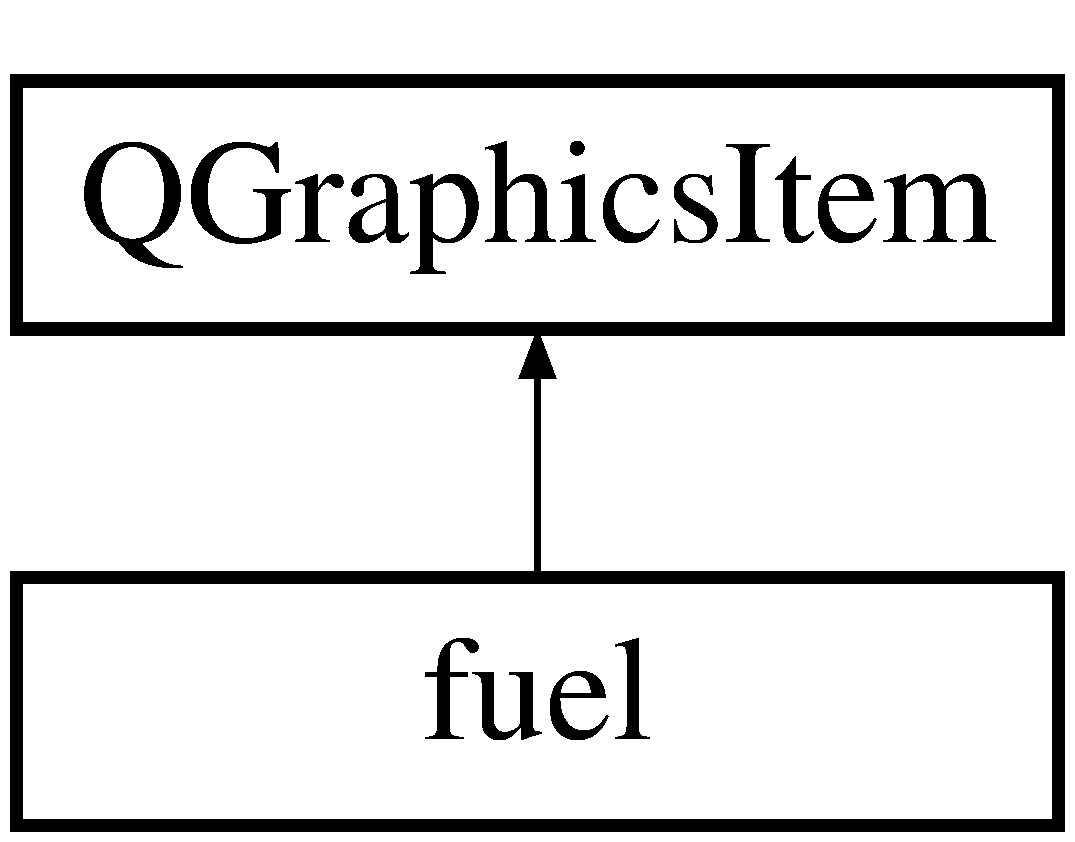
\includegraphics[height=2.000000cm]{classfuel}
\end{center}
\end{figure}
\subsection*{Public Member Functions}
\begin{DoxyCompactItemize}
\item 
\hyperlink{classfuel_ac671922b699142d7f799c4614bb68076}{fuel} (int x, int y, int index, bool direction)
\begin{DoxyCompactList}\small\item\em Fuel objects are collided with and give the alien fuel. \end{DoxyCompactList}\item 
\hypertarget{classfuel_aad4ba33ecb4e9f2fd88a0d833aac4655}{void {\bfseries respawn} ()}\label{classfuel_aad4ba33ecb4e9f2fd88a0d833aac4655}

\end{DoxyCompactItemize}
\subsection*{Protected Member Functions}
\begin{DoxyCompactItemize}
\item 
\hypertarget{classfuel_a48ba549a0290063a1dbcafddb68410a3}{Q\-Rect\-F {\bfseries bounding\-Rect} () const }\label{classfuel_a48ba549a0290063a1dbcafddb68410a3}

\item 
\hypertarget{classfuel_aa65db6b326d7d4408d6de0f8892a9add}{void {\bfseries advance} (int phase)}\label{classfuel_aa65db6b326d7d4408d6de0f8892a9add}

\item 
\hypertarget{classfuel_a102ff178372e69c77d2d71aecfdf38bc}{void {\bfseries paint} (Q\-Painter $\ast$painter, const Q\-Style\-Option\-Graphics\-Item $\ast$option, Q\-Widget $\ast$widget)}\label{classfuel_a102ff178372e69c77d2d71aecfdf38bc}

\end{DoxyCompactItemize}
\subsection*{Private Member Functions}
\begin{DoxyCompactItemize}
\item 
\hypertarget{classfuel_a8cabcfd17b4e025c9943c032d4519344}{void {\bfseries Do\-Collision} ()}\label{classfuel_a8cabcfd17b4e025c9943c032d4519344}

\end{DoxyCompactItemize}
\subsection*{Private Attributes}
\begin{DoxyCompactItemize}
\item 
\hypertarget{classfuel_af3d43e7bbe3d42ece9e044d8ace6bfe6}{qreal {\bfseries starting\-X}}\label{classfuel_af3d43e7bbe3d42ece9e044d8ace6bfe6}

\item 
\hypertarget{classfuel_a22281276336b740787a9df56e5b53615}{qreal {\bfseries starting\-Y}}\label{classfuel_a22281276336b740787a9df56e5b53615}

\item 
\hypertarget{classfuel_aeb782731b4f26cde8299c191cffe1066}{int {\bfseries fuel\-Index}}\label{classfuel_aeb782731b4f26cde8299c191cffe1066}

\item 
\hypertarget{classfuel_af4461708cc91df5f4c022464eaf227a9}{bool {\bfseries fuel\-Direction}}\label{classfuel_af4461708cc91df5f4c022464eaf227a9}

\item 
\hypertarget{classfuel_a0bb7b64595f21fb224541f4921dfa17c}{qreal {\bfseries current\-X}}\label{classfuel_a0bb7b64595f21fb224541f4921dfa17c}

\item 
\hypertarget{classfuel_a63cbdf8f2b0081f1eaee60710fb905f5}{qreal {\bfseries current\-Y}}\label{classfuel_a63cbdf8f2b0081f1eaee60710fb905f5}

\end{DoxyCompactItemize}


\subsection{Constructor \& Destructor Documentation}
\hypertarget{classfuel_ac671922b699142d7f799c4614bb68076}{\index{fuel@{fuel}!fuel@{fuel}}
\index{fuel@{fuel}!fuel@{fuel}}
\subsubsection[{fuel}]{\setlength{\rightskip}{0pt plus 5cm}fuel\-::fuel (
\begin{DoxyParamCaption}
\item[{int}]{x, }
\item[{int}]{y, }
\item[{int}]{index, }
\item[{bool}]{direction}
\end{DoxyParamCaption}
)}}\label{classfuel_ac671922b699142d7f799c4614bb68076}


Fuel objects are collided with and give the alien fuel. 


\begin{DoxyParams}{Parameters}
{\em x} & starting horizontal position \\
\hline
{\em y} & starting vertical position \\
\hline
{\em index} & numerical index \\
\hline
{\em direction} & direction of travel \\
\hline
\end{DoxyParams}


The documentation for this class was generated from the following files\-:\begin{DoxyCompactItemize}
\item 
fuel.\-h\item 
fuel.\-cpp\end{DoxyCompactItemize}

\hypertarget{classgame_label}{\section{game\-Label Class Reference}
\label{classgame_label}\index{game\-Label@{game\-Label}}
}
Inheritance diagram for game\-Label\-:\begin{figure}[H]
\begin{center}
\leavevmode
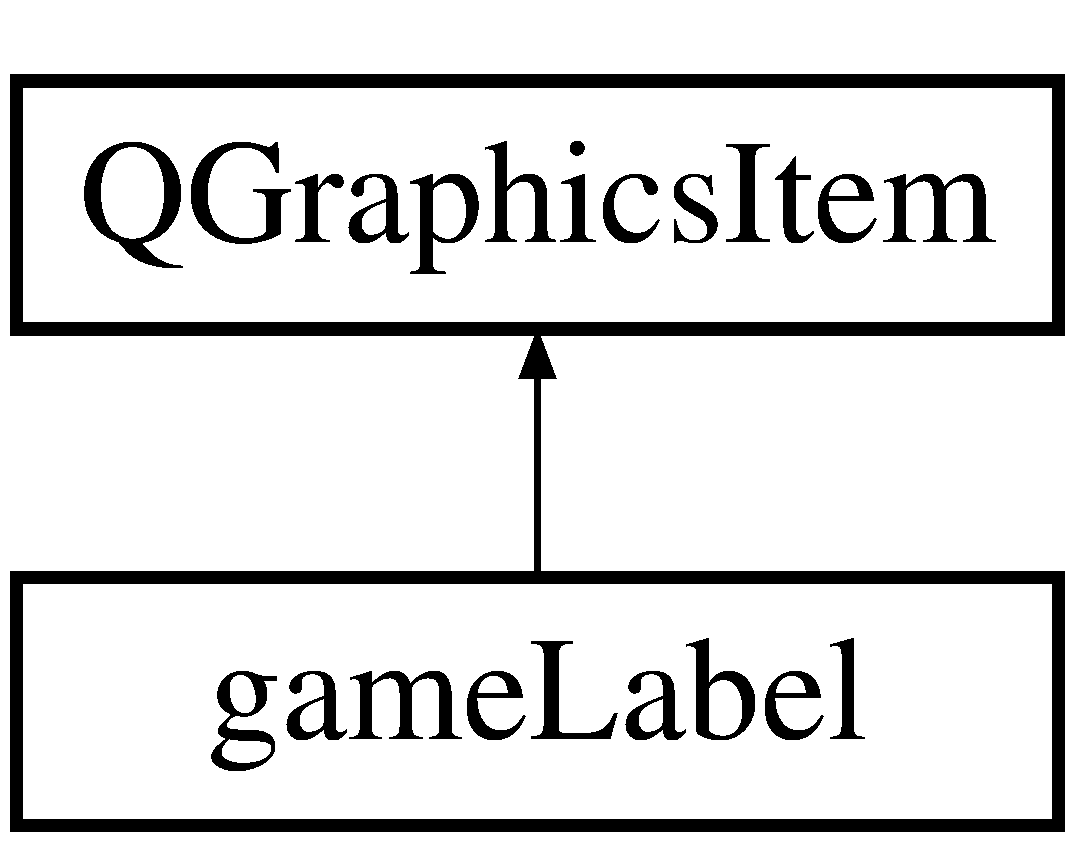
\includegraphics[height=2.000000cm]{classgame_label}
\end{center}
\end{figure}
\subsection*{Public Member Functions}
\begin{DoxyCompactItemize}
\item 
\hyperlink{classgame_label_a9748a8acd420734f3f9292012d466911}{game\-Label} (int x, int y, int index)
\begin{DoxyCompactList}\small\item\em These images are displayed while playing the game. \end{DoxyCompactList}\end{DoxyCompactItemize}
\subsection*{Public Attributes}
\begin{DoxyCompactItemize}
\item 
\hypertarget{classgame_label_a6cef4594f29c0b5b0832ddabdcf27486}{qreal {\bfseries thruster\-Opacity}}\label{classgame_label_a6cef4594f29c0b5b0832ddabdcf27486}

\end{DoxyCompactItemize}
\subsection*{Protected Member Functions}
\begin{DoxyCompactItemize}
\item 
\hypertarget{classgame_label_ac38388c37b084d142c953920fab4d462}{Q\-Rect\-F {\bfseries bounding\-Rect} () const }\label{classgame_label_ac38388c37b084d142c953920fab4d462}

\item 
\hypertarget{classgame_label_a0a0fad187a508d23b7a657a54befd441}{void {\bfseries paint} (Q\-Painter $\ast$painter, const Q\-Style\-Option\-Graphics\-Item $\ast$option, Q\-Widget $\ast$widget)}\label{classgame_label_a0a0fad187a508d23b7a657a54befd441}

\item 
\hypertarget{classgame_label_a652636ae957c00c790cc65ff59cb95c1}{void {\bfseries advance} (int phase)}\label{classgame_label_a652636ae957c00c790cc65ff59cb95c1}

\end{DoxyCompactItemize}
\subsection*{Private Attributes}
\begin{DoxyCompactItemize}
\item 
\hypertarget{classgame_label_ab214bf87e574c8bdadd5215c231d8cc9}{qreal {\bfseries starting\-X}}\label{classgame_label_ab214bf87e574c8bdadd5215c231d8cc9}

\item 
\hypertarget{classgame_label_a00c918e9809be14fc71e249de60bee4c}{qreal {\bfseries starting\-Y}}\label{classgame_label_a00c918e9809be14fc71e249de60bee4c}

\item 
\hypertarget{classgame_label_a400887f564c77170877acade425cbee7}{int {\bfseries game\-Label\-Index}}\label{classgame_label_a400887f564c77170877acade425cbee7}

\end{DoxyCompactItemize}


\subsection{Constructor \& Destructor Documentation}
\hypertarget{classgame_label_a9748a8acd420734f3f9292012d466911}{\index{game\-Label@{game\-Label}!game\-Label@{game\-Label}}
\index{game\-Label@{game\-Label}!gameLabel@{game\-Label}}
\subsubsection[{game\-Label}]{\setlength{\rightskip}{0pt plus 5cm}game\-Label\-::game\-Label (
\begin{DoxyParamCaption}
\item[{int}]{x, }
\item[{int}]{y, }
\item[{int}]{index}
\end{DoxyParamCaption}
)}}\label{classgame_label_a9748a8acd420734f3f9292012d466911}


These images are displayed while playing the game. 


\begin{DoxyParams}{Parameters}
{\em x} & starting horizontal position \\
\hline
{\em y} & starting vertical position \\
\hline
{\em index} & numerical index \\
\hline
\end{DoxyParams}


The documentation for this class was generated from the following files\-:\begin{DoxyCompactItemize}
\item 
gamelabel.\-h\item 
gamelabel.\-cpp\end{DoxyCompactItemize}

\hypertarget{classmineral}{\section{mineral Class Reference}
\label{classmineral}\index{mineral@{mineral}}
}
Inheritance diagram for mineral\-:\begin{figure}[H]
\begin{center}
\leavevmode
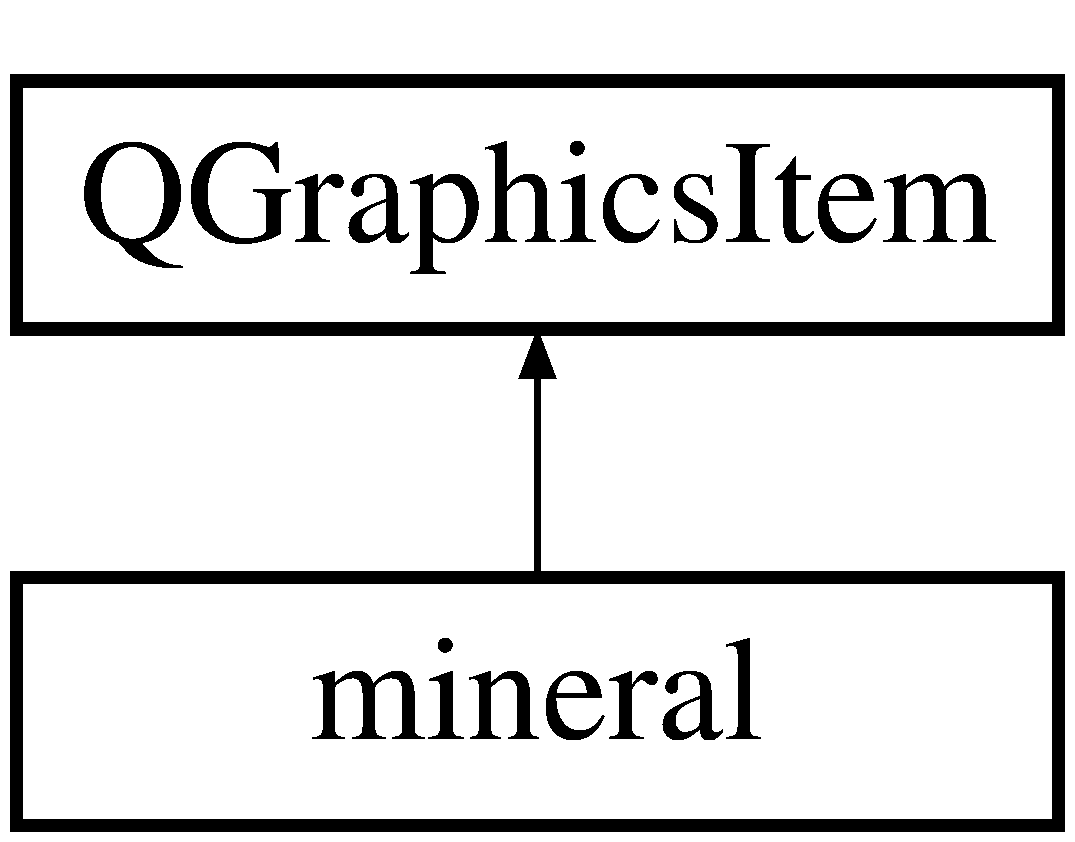
\includegraphics[height=2.000000cm]{classmineral}
\end{center}
\end{figure}
\subsection*{Public Member Functions}
\begin{DoxyCompactItemize}
\item 
\hyperlink{classmineral_ade23474b2da78ce2240dec5341e8cfdf}{mineral} (int x, int y, int index, bool direction)
\begin{DoxyCompactList}\small\item\em Minerals are collided with which give currency. \end{DoxyCompactList}\item 
\hypertarget{classmineral_adc74ea172cd5c998f6255c97e9268100}{void {\bfseries respawn} ()}\label{classmineral_adc74ea172cd5c998f6255c97e9268100}

\end{DoxyCompactItemize}
\subsection*{Public Attributes}
\begin{DoxyCompactItemize}
\item 
\hypertarget{classmineral_a3c1b2c2b147daed638f02af01c14bb75}{bool {\bfseries mineral\-Available}}\label{classmineral_a3c1b2c2b147daed638f02af01c14bb75}

\end{DoxyCompactItemize}
\subsection*{Protected Member Functions}
\begin{DoxyCompactItemize}
\item 
\hypertarget{classmineral_a4e9685fc56fee4b2006ecda5c3d772ea}{Q\-Rect\-F {\bfseries bounding\-Rect} () const }\label{classmineral_a4e9685fc56fee4b2006ecda5c3d772ea}

\item 
\hypertarget{classmineral_a3f644b75e639e41352a174e4fb172735}{void {\bfseries advance} (int phase)}\label{classmineral_a3f644b75e639e41352a174e4fb172735}

\item 
\hypertarget{classmineral_a3246c441cc664188480f47c7197e65ad}{void {\bfseries paint} (Q\-Painter $\ast$painter, const Q\-Style\-Option\-Graphics\-Item $\ast$option, Q\-Widget $\ast$widget)}\label{classmineral_a3246c441cc664188480f47c7197e65ad}

\end{DoxyCompactItemize}
\subsection*{Private Member Functions}
\begin{DoxyCompactItemize}
\item 
\hypertarget{classmineral_a98ab232d582fed02412e8531efb29541}{void {\bfseries Do\-Collision} ()}\label{classmineral_a98ab232d582fed02412e8531efb29541}

\end{DoxyCompactItemize}
\subsection*{Private Attributes}
\begin{DoxyCompactItemize}
\item 
\hypertarget{classmineral_a7b724d02805b0ac5c7c47f4baeeca536}{qreal {\bfseries starting\-X}}\label{classmineral_a7b724d02805b0ac5c7c47f4baeeca536}

\item 
\hypertarget{classmineral_a8921517404d0773bc5924a2ac081c02c}{qreal {\bfseries starting\-Y}}\label{classmineral_a8921517404d0773bc5924a2ac081c02c}

\item 
\hypertarget{classmineral_aefb2a4a4ba71b691cf1071c828745bcc}{int {\bfseries mineral\-Index}}\label{classmineral_aefb2a4a4ba71b691cf1071c828745bcc}

\item 
\hypertarget{classmineral_a0bbaef46590a33fb889ba5a8f9e5ff34}{qreal {\bfseries current\-X}}\label{classmineral_a0bbaef46590a33fb889ba5a8f9e5ff34}

\item 
\hypertarget{classmineral_a386a752f3b90474a767eca7d2b158218}{qreal {\bfseries current\-Y}}\label{classmineral_a386a752f3b90474a767eca7d2b158218}

\end{DoxyCompactItemize}


\subsection{Constructor \& Destructor Documentation}
\hypertarget{classmineral_ade23474b2da78ce2240dec5341e8cfdf}{\index{mineral@{mineral}!mineral@{mineral}}
\index{mineral@{mineral}!mineral@{mineral}}
\subsubsection[{mineral}]{\setlength{\rightskip}{0pt plus 5cm}mineral\-::mineral (
\begin{DoxyParamCaption}
\item[{int}]{x, }
\item[{int}]{y, }
\item[{int}]{index, }
\item[{bool}]{available}
\end{DoxyParamCaption}
)}}\label{classmineral_ade23474b2da78ce2240dec5341e8cfdf}


Minerals are collided with which give currency. 


\begin{DoxyParams}{Parameters}
{\em x} & starting horizontal position \\
\hline
{\em y} & starting vertical position \\
\hline
{\em index} & numerical index \\
\hline
{\em available} & whether or not this mineral is unlocked \\
\hline
\end{DoxyParams}


The documentation for this class was generated from the following files\-:\begin{DoxyCompactItemize}
\item 
mineral.\-h\item 
mineral.\-cpp\end{DoxyCompactItemize}

\hypertarget{classnew_item}{\section{new\-Item Class Reference}
\label{classnew_item}\index{new\-Item@{new\-Item}}
}
Inheritance diagram for new\-Item\-:\begin{figure}[H]
\begin{center}
\leavevmode
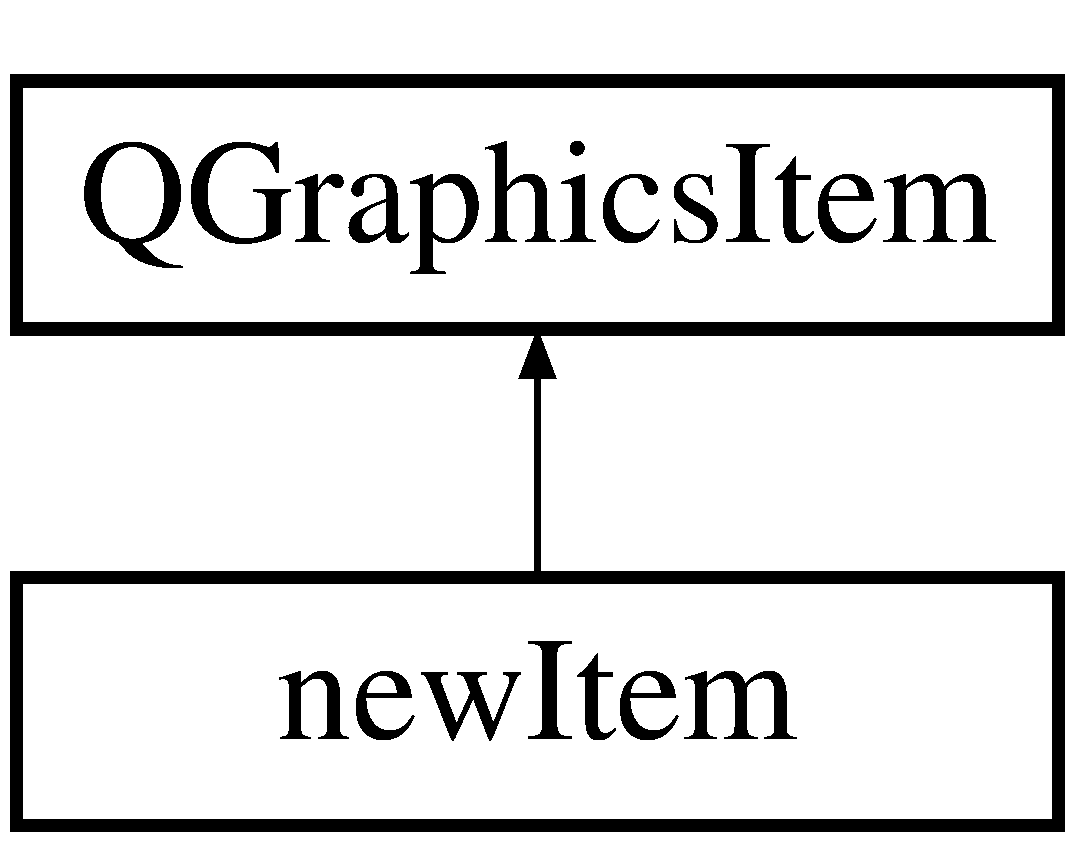
\includegraphics[height=2.000000cm]{classnew_item}
\end{center}
\end{figure}
\subsection*{Public Member Functions}
\begin{DoxyCompactItemize}
\item 
\hypertarget{classnew_item_a108d48d219414392c5052e1b06145565}{\hyperlink{classnew_item_a108d48d219414392c5052e1b06145565}{new\-Item} ()}\label{classnew_item_a108d48d219414392c5052e1b06145565}

\begin{DoxyCompactList}\small\item\em This class represents the aliens attributes and graphical image. \end{DoxyCompactList}\end{DoxyCompactItemize}
\subsection*{Public Attributes}
\begin{DoxyCompactItemize}
\item 
\hypertarget{classnew_item_a5e84dca8f18e29889d1a0ce7c89ca7ef}{bool {\bfseries dead}}\label{classnew_item_a5e84dca8f18e29889d1a0ce7c89ca7ef}

\item 
\hypertarget{classnew_item_af63f68d7216ca8a263ff57125bc6b85f}{qreal {\bfseries lives}}\label{classnew_item_af63f68d7216ca8a263ff57125bc6b85f}

\item 
\hypertarget{classnew_item_a30b397ca477459c46c793b71a806d749}{bool {\bfseries invulnerability}}\label{classnew_item_a30b397ca477459c46c793b71a806d749}

\item 
\hypertarget{classnew_item_aa738e69a3419a355ae20eb91fef66421}{qreal {\bfseries item\-Fuel}}\label{classnew_item_aa738e69a3419a355ae20eb91fef66421}

\item 
\hypertarget{classnew_item_ac94bc2f35eaa0261611a2204ba95d57c}{qreal {\bfseries minerals}}\label{classnew_item_ac94bc2f35eaa0261611a2204ba95d57c}

\item 
\hypertarget{classnew_item_afab8de6447b53884518bb5b12b76685a}{qreal {\bfseries day}}\label{classnew_item_afab8de6447b53884518bb5b12b76685a}

\item 
\hypertarget{classnew_item_adcd13a4a6ebfb2049cb0fa240f7120bf}{bool {\bfseries pet\-Flying}}\label{classnew_item_adcd13a4a6ebfb2049cb0fa240f7120bf}

\item 
\hypertarget{classnew_item_ad135cec328ecd71e02666028d10a8805}{qreal {\bfseries pet\-Bonus}}\label{classnew_item_ad135cec328ecd71e02666028d10a8805}

\item 
\hypertarget{classnew_item_a87f8411c9a808857f83e98327c1572ff}{qreal {\bfseries current\-X}}\label{classnew_item_a87f8411c9a808857f83e98327c1572ff}

\item 
\hypertarget{classnew_item_a8deea72a664e74856e801c0988f866b6}{qreal {\bfseries current\-Y}}\label{classnew_item_a8deea72a664e74856e801c0988f866b6}

\item 
\hypertarget{classnew_item_a14bbd4d47e96e8c959b623f0694cd1bb}{bool {\bfseries dark}}\label{classnew_item_a14bbd4d47e96e8c959b623f0694cd1bb}

\end{DoxyCompactItemize}
\subsection*{Protected Member Functions}
\begin{DoxyCompactItemize}
\item 
\hypertarget{classnew_item_a428251763990e1edf93750f5e922bb2d}{Q\-Rect\-F {\bfseries bounding\-Rect} () const }\label{classnew_item_a428251763990e1edf93750f5e922bb2d}

\item 
\hypertarget{classnew_item_a9df6da5f0b895d1b5d302ce6b7d153bf}{void {\bfseries paint} (Q\-Painter $\ast$painter, const Q\-Style\-Option\-Graphics\-Item $\ast$option, Q\-Widget $\ast$widget)}\label{classnew_item_a9df6da5f0b895d1b5d302ce6b7d153bf}

\item 
\hypertarget{classnew_item_a2da73b26c37070ae64179a45d2fa2f47}{void {\bfseries advance} (int phase)}\label{classnew_item_a2da73b26c37070ae64179a45d2fa2f47}

\end{DoxyCompactItemize}
\subsection*{Private Member Functions}
\begin{DoxyCompactItemize}
\item 
\hypertarget{classnew_item_ac407f5957e6915ba6333ffe03ce0380b}{void {\bfseries Do\-Collision} ()}\label{classnew_item_ac407f5957e6915ba6333ffe03ce0380b}

\end{DoxyCompactItemize}
\subsection*{Private Attributes}
\begin{DoxyCompactItemize}
\item 
\hypertarget{classnew_item_ab37ba167860f718c7c9b0f6889a5c10c}{bool {\bfseries t1}}\label{classnew_item_ab37ba167860f718c7c9b0f6889a5c10c}

\item 
\hypertarget{classnew_item_a850febe1d828ad871e3cd1376e26830c}{bool {\bfseries t2}}\label{classnew_item_a850febe1d828ad871e3cd1376e26830c}

\end{DoxyCompactItemize}


The documentation for this class was generated from the following files\-:\begin{DoxyCompactItemize}
\item 
newitem.\-h\item 
newitem.\-cpp\end{DoxyCompactItemize}

\hypertarget{classpet}{\section{pet Class Reference}
\label{classpet}\index{pet@{pet}}
}
Inheritance diagram for pet\-:\begin{figure}[H]
\begin{center}
\leavevmode
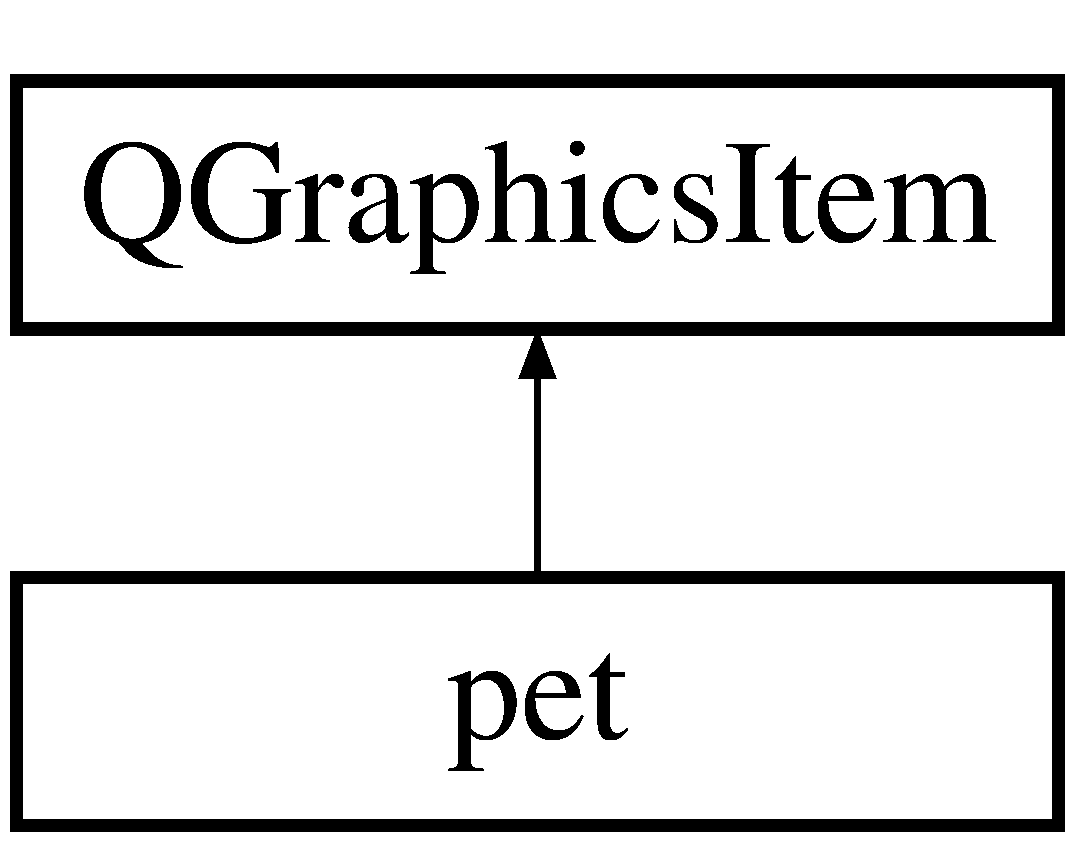
\includegraphics[height=2.000000cm]{classpet}
\end{center}
\end{figure}
\subsection*{Public Member Functions}
\begin{DoxyCompactItemize}
\item 
\hyperlink{classpet_a658aa4452ce51a0b9f7a30855311aaa5}{pet} (int x, int y, int index, bool direction)
\begin{DoxyCompactList}\small\item\em The pet briefly accelerates the background to give the alien speed. \end{DoxyCompactList}\item 
\hypertarget{classpet_a14bbbcb7a01d9c20ccbc3547965291b0}{void {\bfseries respawn} ()}\label{classpet_a14bbbcb7a01d9c20ccbc3547965291b0}

\end{DoxyCompactItemize}
\subsection*{Protected Member Functions}
\begin{DoxyCompactItemize}
\item 
\hypertarget{classpet_ac061847fd6e38d2ef34083da723d85cf}{Q\-Rect\-F {\bfseries bounding\-Rect} () const }\label{classpet_ac061847fd6e38d2ef34083da723d85cf}

\item 
\hypertarget{classpet_a4993baf1888369354747b7df9c6174fd}{void {\bfseries advance} (int phase)}\label{classpet_a4993baf1888369354747b7df9c6174fd}

\item 
\hypertarget{classpet_ac341f1b4ebbc0719e5f65a72306b98f5}{void {\bfseries paint} (Q\-Painter $\ast$painter, const Q\-Style\-Option\-Graphics\-Item $\ast$option, Q\-Widget $\ast$widget)}\label{classpet_ac341f1b4ebbc0719e5f65a72306b98f5}

\end{DoxyCompactItemize}
\subsection*{Private Member Functions}
\begin{DoxyCompactItemize}
\item 
\hypertarget{classpet_af862a4c5e230b358529658e5f9f8615f}{void {\bfseries Do\-Collision} ()}\label{classpet_af862a4c5e230b358529658e5f9f8615f}

\end{DoxyCompactItemize}
\subsection*{Private Attributes}
\begin{DoxyCompactItemize}
\item 
\hypertarget{classpet_a6caa4fe31afe7bcb5325d4568f759e51}{qreal {\bfseries starting\-X}}\label{classpet_a6caa4fe31afe7bcb5325d4568f759e51}

\item 
\hypertarget{classpet_a7aaa8ceec60a3c04c7b3a5c14ebbcd7e}{qreal {\bfseries starting\-Y}}\label{classpet_a7aaa8ceec60a3c04c7b3a5c14ebbcd7e}

\item 
\hypertarget{classpet_a12503937d75d4f86c193251e9c5cd936}{int {\bfseries pet\-Index}}\label{classpet_a12503937d75d4f86c193251e9c5cd936}

\item 
\hypertarget{classpet_a5a874646b211cb361c2e8587d20b87e3}{bool {\bfseries pet\-Direction}}\label{classpet_a5a874646b211cb361c2e8587d20b87e3}

\item 
\hypertarget{classpet_a34b1e23d9bd15d5e319ddfc25f38ad11}{qreal {\bfseries pet\-Speed}}\label{classpet_a34b1e23d9bd15d5e319ddfc25f38ad11}

\item 
\hypertarget{classpet_ab48808361b8fcfeab472b1ec53947251}{qreal {\bfseries current\-X}}\label{classpet_ab48808361b8fcfeab472b1ec53947251}

\item 
\hypertarget{classpet_a9d132e9951b726aa8f24847fe54c7451}{qreal {\bfseries current\-Y}}\label{classpet_a9d132e9951b726aa8f24847fe54c7451}

\end{DoxyCompactItemize}


\subsection{Constructor \& Destructor Documentation}
\hypertarget{classpet_a658aa4452ce51a0b9f7a30855311aaa5}{\index{pet@{pet}!pet@{pet}}
\index{pet@{pet}!pet@{pet}}
\subsubsection[{pet}]{\setlength{\rightskip}{0pt plus 5cm}pet\-::pet (
\begin{DoxyParamCaption}
\item[{int}]{x, }
\item[{int}]{y, }
\item[{int}]{index, }
\item[{bool}]{direction}
\end{DoxyParamCaption}
)}}\label{classpet_a658aa4452ce51a0b9f7a30855311aaa5}


The pet briefly accelerates the background to give the alien speed. 


\begin{DoxyParams}{Parameters}
{\em x} & starting horizontal position \\
\hline
{\em y} & starting vertical position \\
\hline
{\em index} & numerical index \\
\hline
{\em direction} & direction of travel \\
\hline
\end{DoxyParams}


The documentation for this class was generated from the following files\-:\begin{DoxyCompactItemize}
\item 
pet.\-h\item 
pet.\-cpp\end{DoxyCompactItemize}

\hypertarget{classplane}{\section{plane Class Reference}
\label{classplane}\index{plane@{plane}}
}
Inheritance diagram for plane\-:\begin{figure}[H]
\begin{center}
\leavevmode
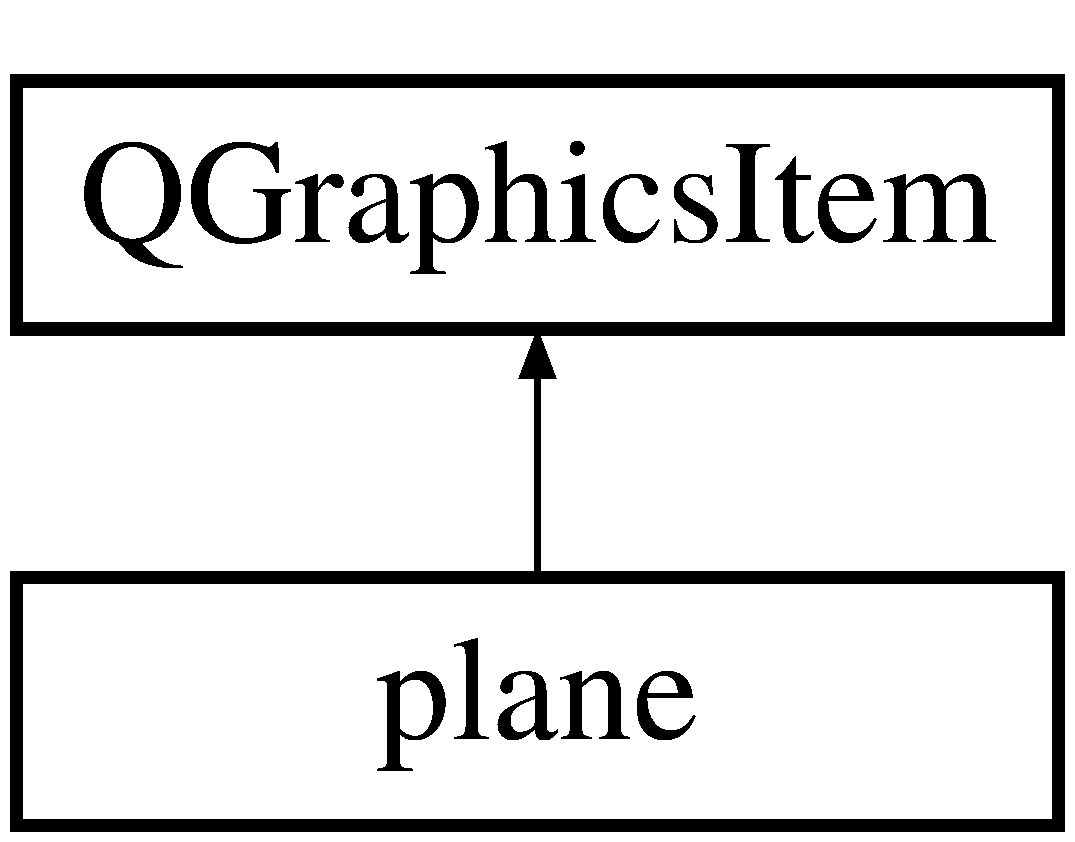
\includegraphics[height=2.000000cm]{classplane}
\end{center}
\end{figure}
\subsection*{Public Member Functions}
\begin{DoxyCompactItemize}
\item 
\hyperlink{classplane_a97cfc3d8bc2aad4732f48f736e4c7e96}{plane} (int x, int y, int index, bool direction)
\begin{DoxyCompactList}\small\item\em Planes collide with the alien to inflict damage. \end{DoxyCompactList}\end{DoxyCompactItemize}
\subsection*{Protected Member Functions}
\begin{DoxyCompactItemize}
\item 
\hypertarget{classplane_a9b1134aa73d32fe993837c31d7a94dd6}{Q\-Rect\-F {\bfseries bounding\-Rect} () const }\label{classplane_a9b1134aa73d32fe993837c31d7a94dd6}

\item 
\hypertarget{classplane_ae3fd03df5b6807372568214b94857e43}{void {\bfseries advance} (int phase)}\label{classplane_ae3fd03df5b6807372568214b94857e43}

\item 
\hypertarget{classplane_a1aaa0881b67ab65d4d088572cc6529c9}{void {\bfseries paint} (Q\-Painter $\ast$painter, const Q\-Style\-Option\-Graphics\-Item $\ast$option, Q\-Widget $\ast$widget)}\label{classplane_a1aaa0881b67ab65d4d088572cc6529c9}

\end{DoxyCompactItemize}
\subsection*{Private Member Functions}
\begin{DoxyCompactItemize}
\item 
\hypertarget{classplane_a5b8c6d5ad84af4efb64ca3b9536bf071}{void {\bfseries Do\-Collision} ()}\label{classplane_a5b8c6d5ad84af4efb64ca3b9536bf071}

\end{DoxyCompactItemize}
\subsection*{Private Attributes}
\begin{DoxyCompactItemize}
\item 
\hypertarget{classplane_aaf522b494e4d68ccb5fe0614423ab8f9}{qreal {\bfseries starting\-X}}\label{classplane_aaf522b494e4d68ccb5fe0614423ab8f9}

\item 
\hypertarget{classplane_a1703e83da5bec6e4fcb6e5a55051ee0b}{qreal {\bfseries starting\-Y}}\label{classplane_a1703e83da5bec6e4fcb6e5a55051ee0b}

\item 
\hypertarget{classplane_aa424008b51f90740a2946190225ff911}{int {\bfseries plane\-Index}}\label{classplane_aa424008b51f90740a2946190225ff911}

\item 
\hypertarget{classplane_a44ad410c8f2d8417f50f9d3c691ac0fc}{bool {\bfseries plane\-Direction}}\label{classplane_a44ad410c8f2d8417f50f9d3c691ac0fc}

\item 
\hypertarget{classplane_a65b10df1c12caae50651103b209551c8}{qreal {\bfseries current\-X}}\label{classplane_a65b10df1c12caae50651103b209551c8}

\item 
\hypertarget{classplane_ae83d7dc07caed31cfff48d92f98d8ffa}{qreal {\bfseries current\-Y}}\label{classplane_ae83d7dc07caed31cfff48d92f98d8ffa}

\item 
\hypertarget{classplane_ad64ebf01deae230942cb32a9e6e00a2d}{qreal {\bfseries plane\-Speed}}\label{classplane_ad64ebf01deae230942cb32a9e6e00a2d}

\end{DoxyCompactItemize}


\subsection{Constructor \& Destructor Documentation}
\hypertarget{classplane_a97cfc3d8bc2aad4732f48f736e4c7e96}{\index{plane@{plane}!plane@{plane}}
\index{plane@{plane}!plane@{plane}}
\subsubsection[{plane}]{\setlength{\rightskip}{0pt plus 5cm}plane\-::plane (
\begin{DoxyParamCaption}
\item[{int}]{x, }
\item[{int}]{y, }
\item[{int}]{index, }
\item[{bool}]{direction}
\end{DoxyParamCaption}
)}}\label{classplane_a97cfc3d8bc2aad4732f48f736e4c7e96}


Planes collide with the alien to inflict damage. 


\begin{DoxyParams}{Parameters}
{\em x} & starting horizontal position \\
\hline
{\em y} & starting vertical position \\
\hline
{\em index} & numerical index \\
\hline
{\em direction} & direction of travel \\
\hline
\end{DoxyParams}


The documentation for this class was generated from the following files\-:\begin{DoxyCompactItemize}
\item 
plane.\-h\item 
plane.\-cpp\end{DoxyCompactItemize}

\hypertarget{classscript}{\section{script Class Reference}
\label{classscript}\index{script@{script}}
}
Inheritance diagram for script\-:\begin{figure}[H]
\begin{center}
\leavevmode
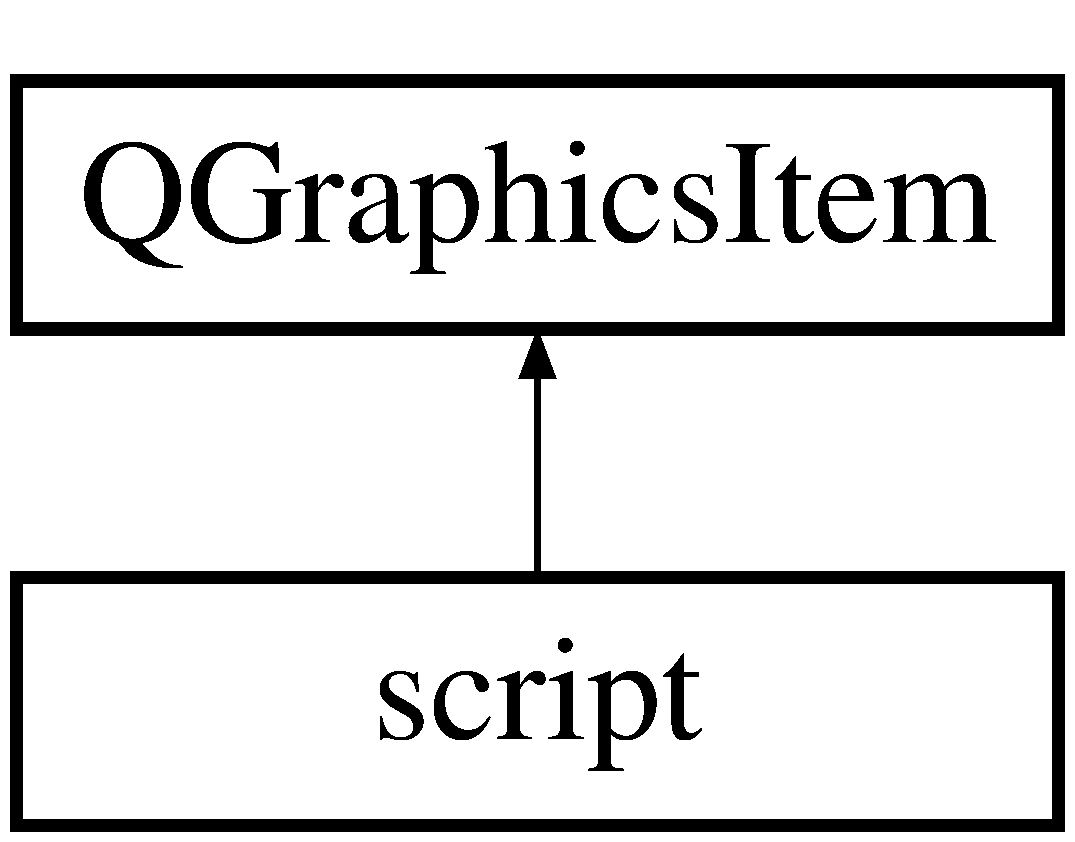
\includegraphics[height=2.000000cm]{classscript}
\end{center}
\end{figure}
\subsection*{Public Member Functions}
\begin{DoxyCompactItemize}
\item 
\hyperlink{classscript_aa086f1b44018c0317df0bcd6a3d09e4e}{script} (int x, int y, int o)
\begin{DoxyCompactList}\small\item\em This class represents the text before the game starts. \end{DoxyCompactList}\end{DoxyCompactItemize}
\subsection*{Public Attributes}
\begin{DoxyCompactItemize}
\item 
\hypertarget{classscript_a831f3571933acedf6b0bc9e4759a3c1d}{qreal {\bfseries order}}\label{classscript_a831f3571933acedf6b0bc9e4759a3c1d}

\item 
\hypertarget{classscript_a04e0af34c71aebcb4f37c743c4a597e0}{qreal {\bfseries counter}}\label{classscript_a04e0af34c71aebcb4f37c743c4a597e0}

\end{DoxyCompactItemize}
\subsection*{Protected Member Functions}
\begin{DoxyCompactItemize}
\item 
\hypertarget{classscript_a994bf028612ab2af537bbb660ce82315}{Q\-Rect\-F {\bfseries bounding\-Rect} () const }\label{classscript_a994bf028612ab2af537bbb660ce82315}

\item 
\hypertarget{classscript_a3f01cd4e6af8a4c7a9e7d94d416715dc}{void {\bfseries paint} (Q\-Painter $\ast$painter, const Q\-Style\-Option\-Graphics\-Item $\ast$option, Q\-Widget $\ast$widget)}\label{classscript_a3f01cd4e6af8a4c7a9e7d94d416715dc}

\item 
\hypertarget{classscript_a4c0dac2338f5431969dbb72e1851720f}{void {\bfseries advance} (int phase)}\label{classscript_a4c0dac2338f5431969dbb72e1851720f}

\end{DoxyCompactItemize}
\subsection*{Private Attributes}
\begin{DoxyCompactItemize}
\item 
\hypertarget{classscript_af2c4d96e769bfa9dbf391158e331a735}{qreal {\bfseries starting\-X}}\label{classscript_af2c4d96e769bfa9dbf391158e331a735}

\item 
\hypertarget{classscript_a9353463dc99349444713d6a475ff7581}{qreal {\bfseries starting\-Y}}\label{classscript_a9353463dc99349444713d6a475ff7581}

\end{DoxyCompactItemize}


\subsection{Constructor \& Destructor Documentation}
\hypertarget{classscript_aa086f1b44018c0317df0bcd6a3d09e4e}{\index{script@{script}!script@{script}}
\index{script@{script}!script@{script}}
\subsubsection[{script}]{\setlength{\rightskip}{0pt plus 5cm}script\-::script (
\begin{DoxyParamCaption}
\item[{int}]{x, }
\item[{int}]{y, }
\item[{int}]{o}
\end{DoxyParamCaption}
)}}\label{classscript_aa086f1b44018c0317df0bcd6a3d09e4e}


This class represents the text before the game starts. 


\begin{DoxyParams}{Parameters}
{\em x} & starting horizontal position \\
\hline
{\em y} & starting vertical position \\
\hline
{\em o} & order of presentation (1 or 2) \\
\hline
\end{DoxyParams}


The documentation for this class was generated from the following files\-:\begin{DoxyCompactItemize}
\item 
script.\-h\item 
script.\-cpp\end{DoxyCompactItemize}

\hypertarget{classship}{\section{ship Class Reference}
\label{classship}\index{ship@{ship}}
}
Inheritance diagram for ship\-:\begin{figure}[H]
\begin{center}
\leavevmode
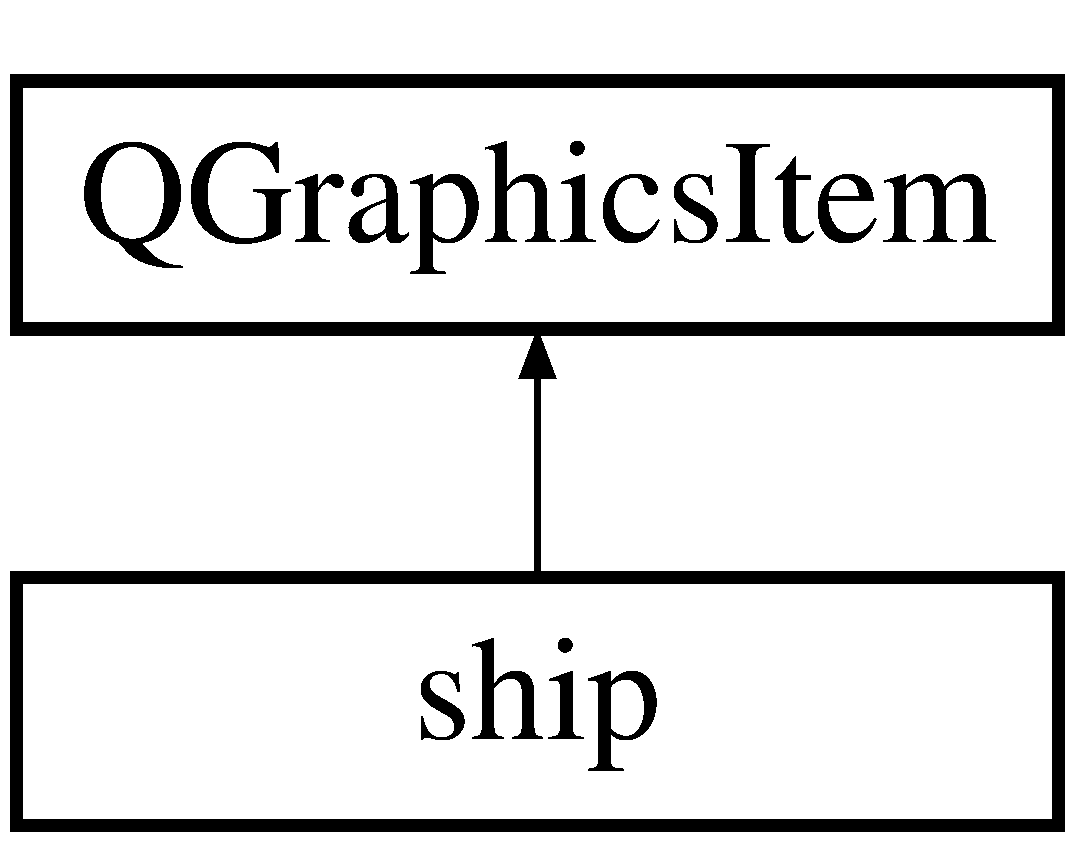
\includegraphics[height=2.000000cm]{classship}
\end{center}
\end{figure}
\subsection*{Public Member Functions}
\begin{DoxyCompactItemize}
\item 
\hypertarget{classship_a002c8f2eea35e3b4f0c8003850a782d4}{\hyperlink{classship_a002c8f2eea35e3b4f0c8003850a782d4}{ship} ()}\label{classship_a002c8f2eea35e3b4f0c8003850a782d4}

\begin{DoxyCompactList}\small\item\em Colliding with the ship is the win condition for the game. \end{DoxyCompactList}\end{DoxyCompactItemize}
\subsection*{Protected Member Functions}
\begin{DoxyCompactItemize}
\item 
\hypertarget{classship_a4941ffe7e91c54d95aec7fcd32e1bc2f}{Q\-Rect\-F {\bfseries bounding\-Rect} () const }\label{classship_a4941ffe7e91c54d95aec7fcd32e1bc2f}

\item 
\hypertarget{classship_a07a6cb76b7b3b96ac3617fc12cdc786a}{void {\bfseries paint} (Q\-Painter $\ast$painter, const Q\-Style\-Option\-Graphics\-Item $\ast$option, Q\-Widget $\ast$widget)}\label{classship_a07a6cb76b7b3b96ac3617fc12cdc786a}

\end{DoxyCompactItemize}
\subsection*{Private Member Functions}
\begin{DoxyCompactItemize}
\item 
\hypertarget{classship_ab9d36b37f61a759bd8fa62cb12d7de2d}{void {\bfseries Do\-Collision} ()}\label{classship_ab9d36b37f61a759bd8fa62cb12d7de2d}

\end{DoxyCompactItemize}
\subsection*{Private Attributes}
\begin{DoxyCompactItemize}
\item 
\hypertarget{classship_abd81a1e65e3a5eb6bff09c804b418187}{Q\-String {\bfseries str\-\_\-win}}\label{classship_abd81a1e65e3a5eb6bff09c804b418187}

\end{DoxyCompactItemize}


The documentation for this class was generated from the following files\-:\begin{DoxyCompactItemize}
\item 
ship.\-h\item 
ship.\-cpp\end{DoxyCompactItemize}

\hypertarget{classupgrade}{\section{upgrade Class Reference}
\label{classupgrade}\index{upgrade@{upgrade}}
}
Inheritance diagram for upgrade\-:\begin{figure}[H]
\begin{center}
\leavevmode
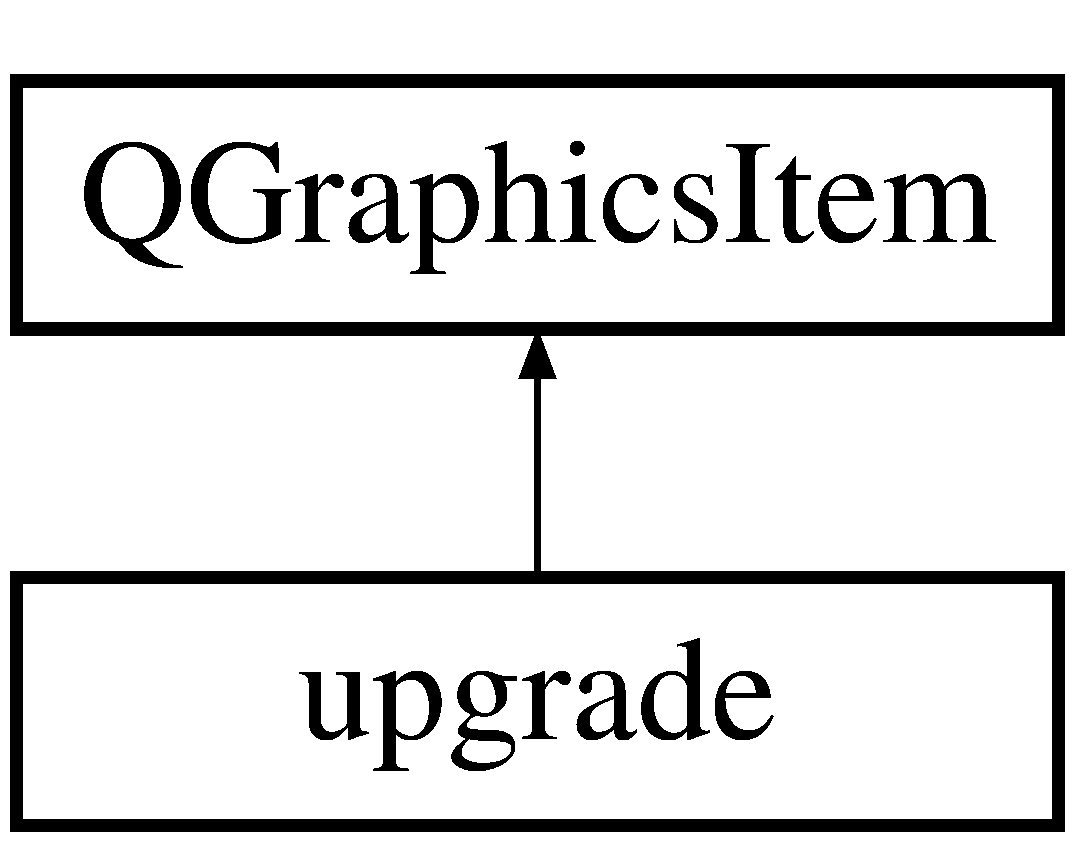
\includegraphics[height=2.000000cm]{classupgrade}
\end{center}
\end{figure}
\subsection*{Public Member Functions}
\begin{DoxyCompactItemize}
\item 
\hypertarget{classupgrade_af4629a61539fd8bfa371b625a85041c8}{void {\bfseries blackout\-Start} ()}\label{classupgrade_af4629a61539fd8bfa371b625a85041c8}

\item 
\hyperlink{classupgrade_adb0c00eec47ddfd36b00713659e09141}{upgrade} (int index)
\begin{DoxyCompactList}\small\item\em These objects are clickable and represent the vairious possible upgrades you can purchase. \end{DoxyCompactList}\end{DoxyCompactItemize}
\subsection*{Public Attributes}
\begin{DoxyCompactItemize}
\item 
\hypertarget{classupgrade_a8a08f313ef51624c733fabff824ae2b6}{int {\bfseries upgrade\-\_\-level}}\label{classupgrade_a8a08f313ef51624c733fabff824ae2b6}

\end{DoxyCompactItemize}
\subsection*{Protected Member Functions}
\begin{DoxyCompactItemize}
\item 
\hypertarget{classupgrade_a3fedbd880be00ca2681acf29001a632b}{Q\-Rect\-F {\bfseries bounding\-Rect} () const }\label{classupgrade_a3fedbd880be00ca2681acf29001a632b}

\item 
\hypertarget{classupgrade_a3321bc5f314d7e69a9b6ead5a4a971ea}{void {\bfseries advance} (int phase)}\label{classupgrade_a3321bc5f314d7e69a9b6ead5a4a971ea}

\item 
\hypertarget{classupgrade_aa391e458dc162a19da4ef4518c41f314}{void {\bfseries paint} (Q\-Painter $\ast$painter, const Q\-Style\-Option\-Graphics\-Item $\ast$option, Q\-Widget $\ast$widget)}\label{classupgrade_aa391e458dc162a19da4ef4518c41f314}

\end{DoxyCompactItemize}
\subsection*{Private Attributes}
\begin{DoxyCompactItemize}
\item 
\hypertarget{classupgrade_a4eba65a9c67f04d342e7318aa3d754a3}{int {\bfseries img\-\_\-index}}\label{classupgrade_a4eba65a9c67f04d342e7318aa3d754a3}

\item 
\hypertarget{classupgrade_a4e395982c4ca51eca479446cf38f56e6}{Q\-String {\bfseries str}}\label{classupgrade_a4e395982c4ca51eca479446cf38f56e6}

\item 
\hypertarget{classupgrade_a3462cd477a633ad53a81d81c617f4548}{bool {\bfseries min\-Count\-Init}}\label{classupgrade_a3462cd477a633ad53a81d81c617f4548}

\end{DoxyCompactItemize}


\subsection{Constructor \& Destructor Documentation}
\hypertarget{classupgrade_adb0c00eec47ddfd36b00713659e09141}{\index{upgrade@{upgrade}!upgrade@{upgrade}}
\index{upgrade@{upgrade}!upgrade@{upgrade}}
\subsubsection[{upgrade}]{\setlength{\rightskip}{0pt plus 5cm}upgrade\-::upgrade (
\begin{DoxyParamCaption}
\item[{int}]{index}
\end{DoxyParamCaption}
)}}\label{classupgrade_adb0c00eec47ddfd36b00713659e09141}


These objects are clickable and represent the vairious possible upgrades you can purchase. 


\begin{DoxyParams}{Parameters}
{\em index} & numerical index \\
\hline
\end{DoxyParams}


The documentation for this class was generated from the following files\-:\begin{DoxyCompactItemize}
\item 
upgrade.\-h\item 
upgrade.\-cpp\end{DoxyCompactItemize}

%--- End generated contents ---

% Index
\newpage
\phantomsection
\addcontentsline{toc}{part}{Index}
\printindex

\end{document}
